\documentclass[dvipdfmx,12pt]{beamer}

\usepackage{bxdpx-beamer}
\usepackage{pxjahyper}
\usepackage{minijs}
\usetheme{Annarbor}
\usepackage{mathpazo}
\usepackage{amsmath,amssymb}
\usepackage{graphicx}
\usepackage{array}
\usepackage{tikz}

\title{Reference dependent preference, but whose?}
\subtitle{Evidence from MLB batters}
\author{Reio TANJI}
\date{Oct 2 2018}
\institute{Osaka University}

\begin{document}
\begin{frame}\frametitle{}
\titlepage
\end{frame}

\begin{frame}\frametitle{Abstract}
  \begin{itemize}
    \item Specify the reference-dependent preference of the baseball
    players (Position players) by the econometric analysis

    \item Players regard the 0.300 \textit{Batting average}
    as reference point and for many cases succesfully meet their goals.

    \item This tendency is observed only in .300 of Batting-Average,
    not in other round numbers (e.g. .200, .250) or other
    performance statistics, such as On-Base Percentage (: Rate statistics)
     or Homeruns (Cumulative statistics).

    \item There seems to be no monetary incentives for the players to do so.
  \end{itemize}
\end{frame}

\section*{A Table of Contents}
\begin{frame}\frametitle{Contents}
 \tableofcontents
\end{frame}

\section{Introduction}
\begin{frame}\frametitle{Literature}
  \begin{itemize}
    \item Pope \& Simonsohn (2011) picked up MLB batters as an empirical evidence
    of ``Round number reference dependence. ``

    : They showed excess distribution above .300 of batting-average.

     \begin{figure}
       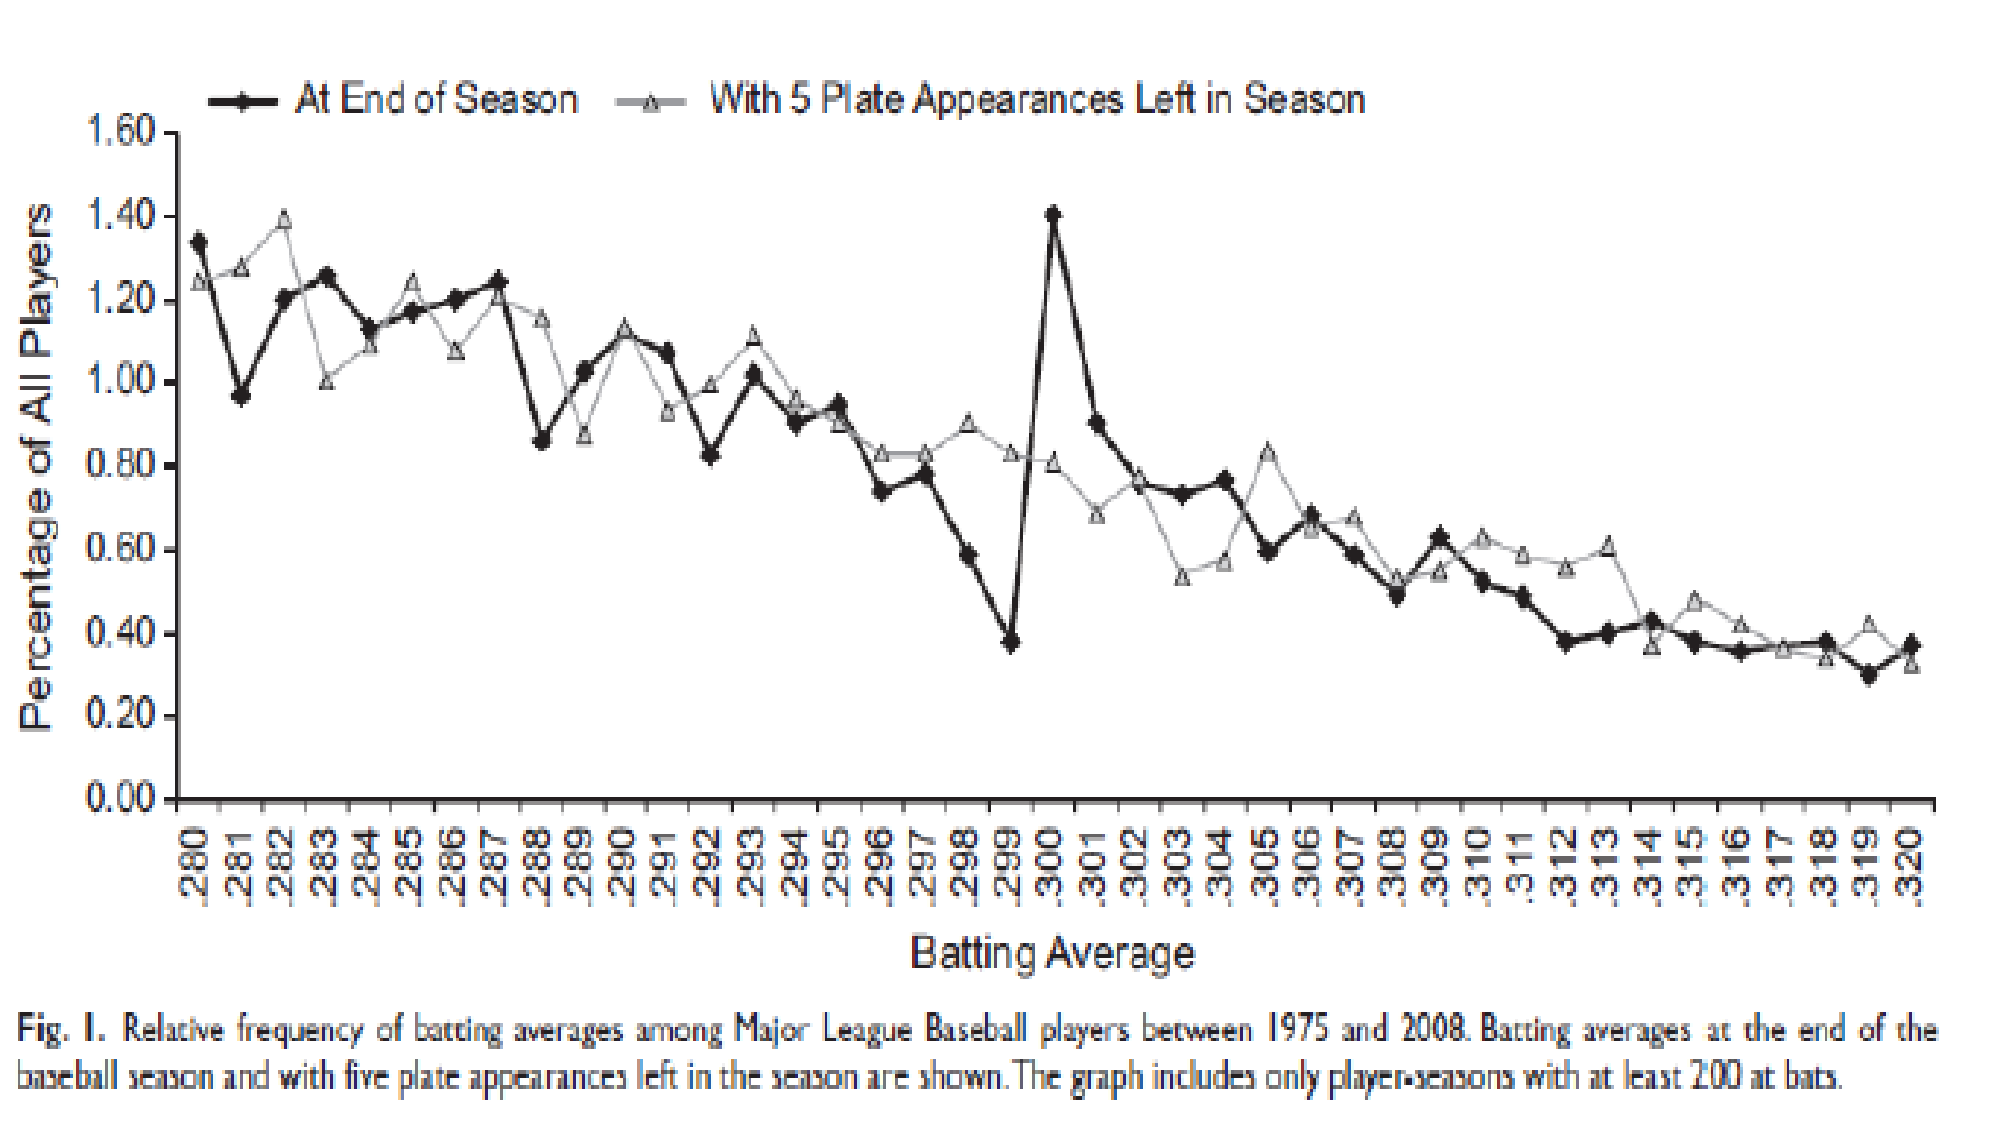
\includegraphics[width = 8cm, height = 5cm]{fig_tab/mt_fig1.pdf}
     \end{figure}
  \end{itemize}
\end{frame}

\begin{frame}\frametitle{Literature}
  \begin{itemize}
    \item Allen et al. (2016) emphasized the existence of the round number
    reference point dependence of the marathon runners' finishing times.

    \begin{figure}
      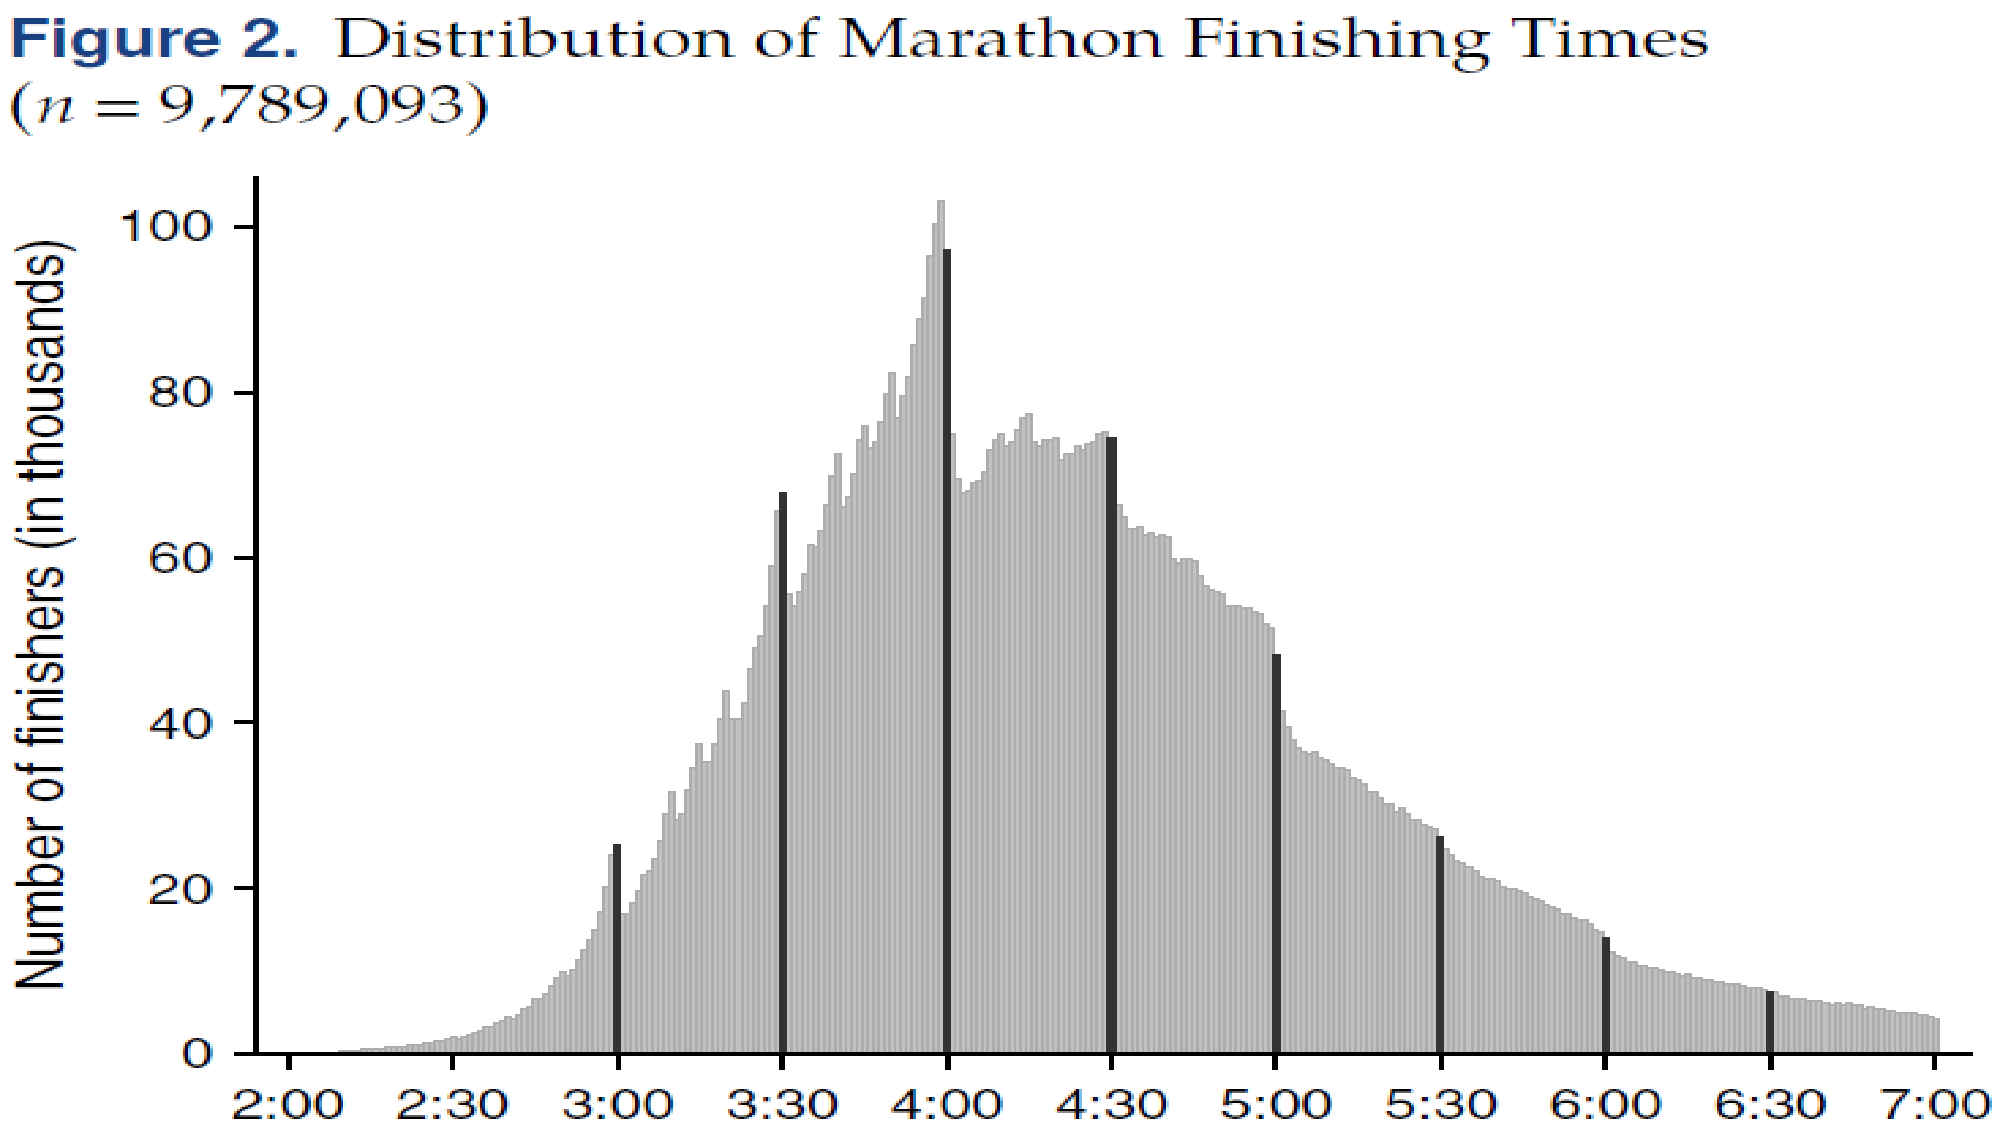
\includegraphics[width = 6.3cm, height = 5.5cm]{fig_tab/mt_fig2.pdf}
    \end{figure}
  \end{itemize}
\end{frame}

\begin{frame}\frametitle{Research Question}
  \begin{itemize}
    \item In this study, I conducted further research in three view points.
    \begin{enumerate}
      \item Does round-number dependent preference occur in other statistics?

      : difference between ``rate statistics`` and ``cumulative statistics``

      \item Is the reference dependent preference actually the player's?

      : If there is \textit{monetary incentive} for the players to try to
      meet the goals, then it may be the team manager that has reference
      dependence.

      \item What about when the relative importance of batting-average
      diminishes?

      : The publication of `\textit{Moneyball}` has been change the evaluation
      of the people about the importance of batting average.
    \end{enumerate}
  \end{itemize}
\end{frame}

\section{Framework}
\begin{frame}\frametitle{Theoretical Framework}
  \begin{itemize}
    \item Primary gain-loss function:Kahneman \& Tversky(1979)

    \[ V(x|r) = \begin{cases}
    v(x - r) & \text{ if } x \geq r \\
    - \lambda v (x - r) & \text{ if } x < r
    \end{cases} \]

   \item In this research, I follow utilize the specification
   of Allen et al. (2016), discontinuity at the reference point:
   \[ \lim_{\epsilon \to 0} v(r + \epsilon) \neq
   \lim_{\epsilon \to 0} v(r - \epsilon)
   \]
  \end{itemize}
\end{frame}

\begin{frame}\frametitle{Theoretical Framework}
 \begin{itemize}
   \item utility function with discontinuity at the reference point
    \begin{tikzpicture}[domain = 0:4, samples = 200, >= stealth]
      \draw[->](-0.5, 0) -- (4.2, 0) node[right]{$x$};
      \draw[->](0, -0.5) -- (0, 2.2) node[above]{$v(x)$};
      \draw[-](2.2, -0.1) -- (2.2, 0.1);
      \draw[domain=0:2.2,samples=200,>=stealth] plot (\x, {sqrt(\x)});
      \draw[domain=2.2:4.1,samples=200,>=stealth] plot (\x, {sqrt(\x) + 0.3});
      \draw (0, 0) node[below left]{O};
      \draw (2.2, -0.3) node {$r$};
    \end{tikzpicture}
  \item This utility function makes
  \begin{itemize}
    \item players try to meet their goals and excess distribution around the reference
    point observed
    \item team managers overestimate whether he achieves to reach above the
    reference point.
  \end{itemize}
 \end{itemize}

\end{frame}

\section{Empirical Method and Data}

\begin{frame}\frametitle{Method: Monetary incentives}
 \begin{align*}
   w_{it} = \beta_0 & X_{it} + \beta_1 \text{ABOVE300}_{it} \\
   & + \beta_2 X_{it} \times \text{ABOVE300}_{it} + \beta_3 Z_{it} \\
   \text{where} \\
  w_{it}:& \text{Log-salary of the player } i \text{ in } t+1 \text{ season} \\
  X_{it}:& \text{Proxy for the performance of the player} \\
  \text{ABOVE}:& \text{indicator if the player achieves their inferred goals} \\
  Z_{it}:& \text{Player-specific charactaristics}
 \end{align*}
\end{frame}

\begin{frame}\frametitle{Data Description}
\begin{itemize}
  \item Panel data of the player performance and salary.
  \begin{itemize}
    \item Various performance statistics tagged by the player ID and year
    from ``fangraphs'' (1957 to 2017, $n=53,090 (61 \text{ seasons})$)

    \item Salary data from USA TODAY (1987 to 2017, $n=8,928$ (31 seasons))

  \end{itemize}

  \item Time-series data of team performance statistics (1987 to 2017, 31 seasons)
  from ``Baseball reference.''
\end{itemize}
\end{frame}

\begin{frame}\frametitle{Definitions of Statistics}
 \footnotesize
 \begin{itemize}
   \item Batting-Average (AVG)
    \[
    \text{AVG} = \text{Base-Hit}/\text{At-Bat}
    \]
   \item On-Base Percentage (OBP)
    \[
    \text{OBP} = \dfrac{\text{Base-Hit} + \text{Walk} + \text{Hit-by-Pitch}}{
    \text{Prate-Appearance} - \text{Sacrifice-Hit} - \text{Catcher-Interferance}
    }
    \]
    \item Slugging Average (SLG)
    \[\text{SLG} = \dfrac{\text{Single} + 2 \times \text{Double} + 3 \times
    \text{Triple} + 4 \times \text{HR}}{\text{At-Bat}}
    \]
 \end{itemize}
\end{frame}

\section{Results}
\begin{frame}
  \begin{figure}
    \centering
    \includegraphics[width = 8.4cm, height = 6cm]
    {C:/Users/T-Reio/Master_thesis/master_thesis/graphs/AVG_200PA.png}
\label{AVG}
    \footnotesize

    *difference between the number of batters with .299 (0.37\%)
     and .300 (1.13\%) is significant at 0.1\% ($\chi^2 = 69.03$)

     **Also, the difference between those with .299, .298 (0.87\%)
     and with .300 and .301 (1.91\%) is significant at 0.1\%
     ($\chi^2 = 70.26$)
  \end{figure}
\end{frame}
\begin{frame}
  Other statistics: Rate statistics
  \begin{figure}
    \centering
    \includegraphics[width = 8.4cm, height = 6cm]
      {C:/Users/T-Reio/Master_thesis/master_thesis/graphs/OBP_200PA.png}
    \footnotesize

    There was no observation of round number dependence.

    OPS (OBP + SLG) either does not show such tendency.
\label{OBP}
  \end{figure}
\end{frame}

\begin{frame}
 Other statistics: Cumulative statistics
 \begin{figure}
   \centering
   \includegraphics[width = 8.4cm, height = 6cm]
   {C:/Users/T-Reio/Master_thesis/master_thesis/graphs/H_90PA.png}
   \footnotesize

   Also, round number reference dependence is not observed.

\label{Base-Hit}
 \end{figure}
\end{frame}

\begin{frame}
  \begin{figure}
    \includegraphics[width = 8.4cm, height = 6cm]
    {C:/Users/T-Reio/Master_thesis/master_thesis/graphs/SB_5SB.png}

    \footnotesize
    Stolen-Bases may be more easily controled, but no reference-dependence
    observed.
\label{Stolen-Bases}
  \end{figure}
\end{frame}

\begin{frame}\frametitle{Observed Choice of the player}
 \begin{itemize}
   \item .300 of AVG seems to act as a reference point, but it may not be
   ``round number" dependence, as is mentioned in Pope \& Simonsohn (2011)

   \item Such a behavior is observed only in AVG, not in either rate statistics
   or cumulative ones.

   \item Then, we next have to see whether there is some monetary incentives
   for the player, which reveals that the observed behavior is certainly
   the player's preference.

 \end{itemize}
\end{frame}

\begin{frame}\frametitle{Measuring Performance}
  \begin{itemize}
    \item In the regression analysis, I utilize the statistics below as
    proxies for performance:
    \begin{itemize}
      \footnotesize
      \item Weighted On-base Percentage (wOBA)

      : Value of runs the batter produce per plate-appearance (+ adjustment)

      \item BATTING, FIELDING and BaseRun

      : Runs created by the batter by batting, fielding and baserunning,
       respectively.

      \item (fangraphs) Win-above-Replacement (fWAR)

      : Wins created by the player, relative to the ``replacement level" player,
      who has value as a player that achieves .298 of win-average.

      \item (negative) Win-Probability Added (WPA (nWPA))

      : Sum of how much their action increased (decreased)
      their team’s odds of winning

      In this research, I devide this with the number of games he attended.
    \end{itemize}
  \end{itemize}
\end{frame}

\begin{frame}
  \scriptsize
  Comparision among various statistics

 \begin{figure}
   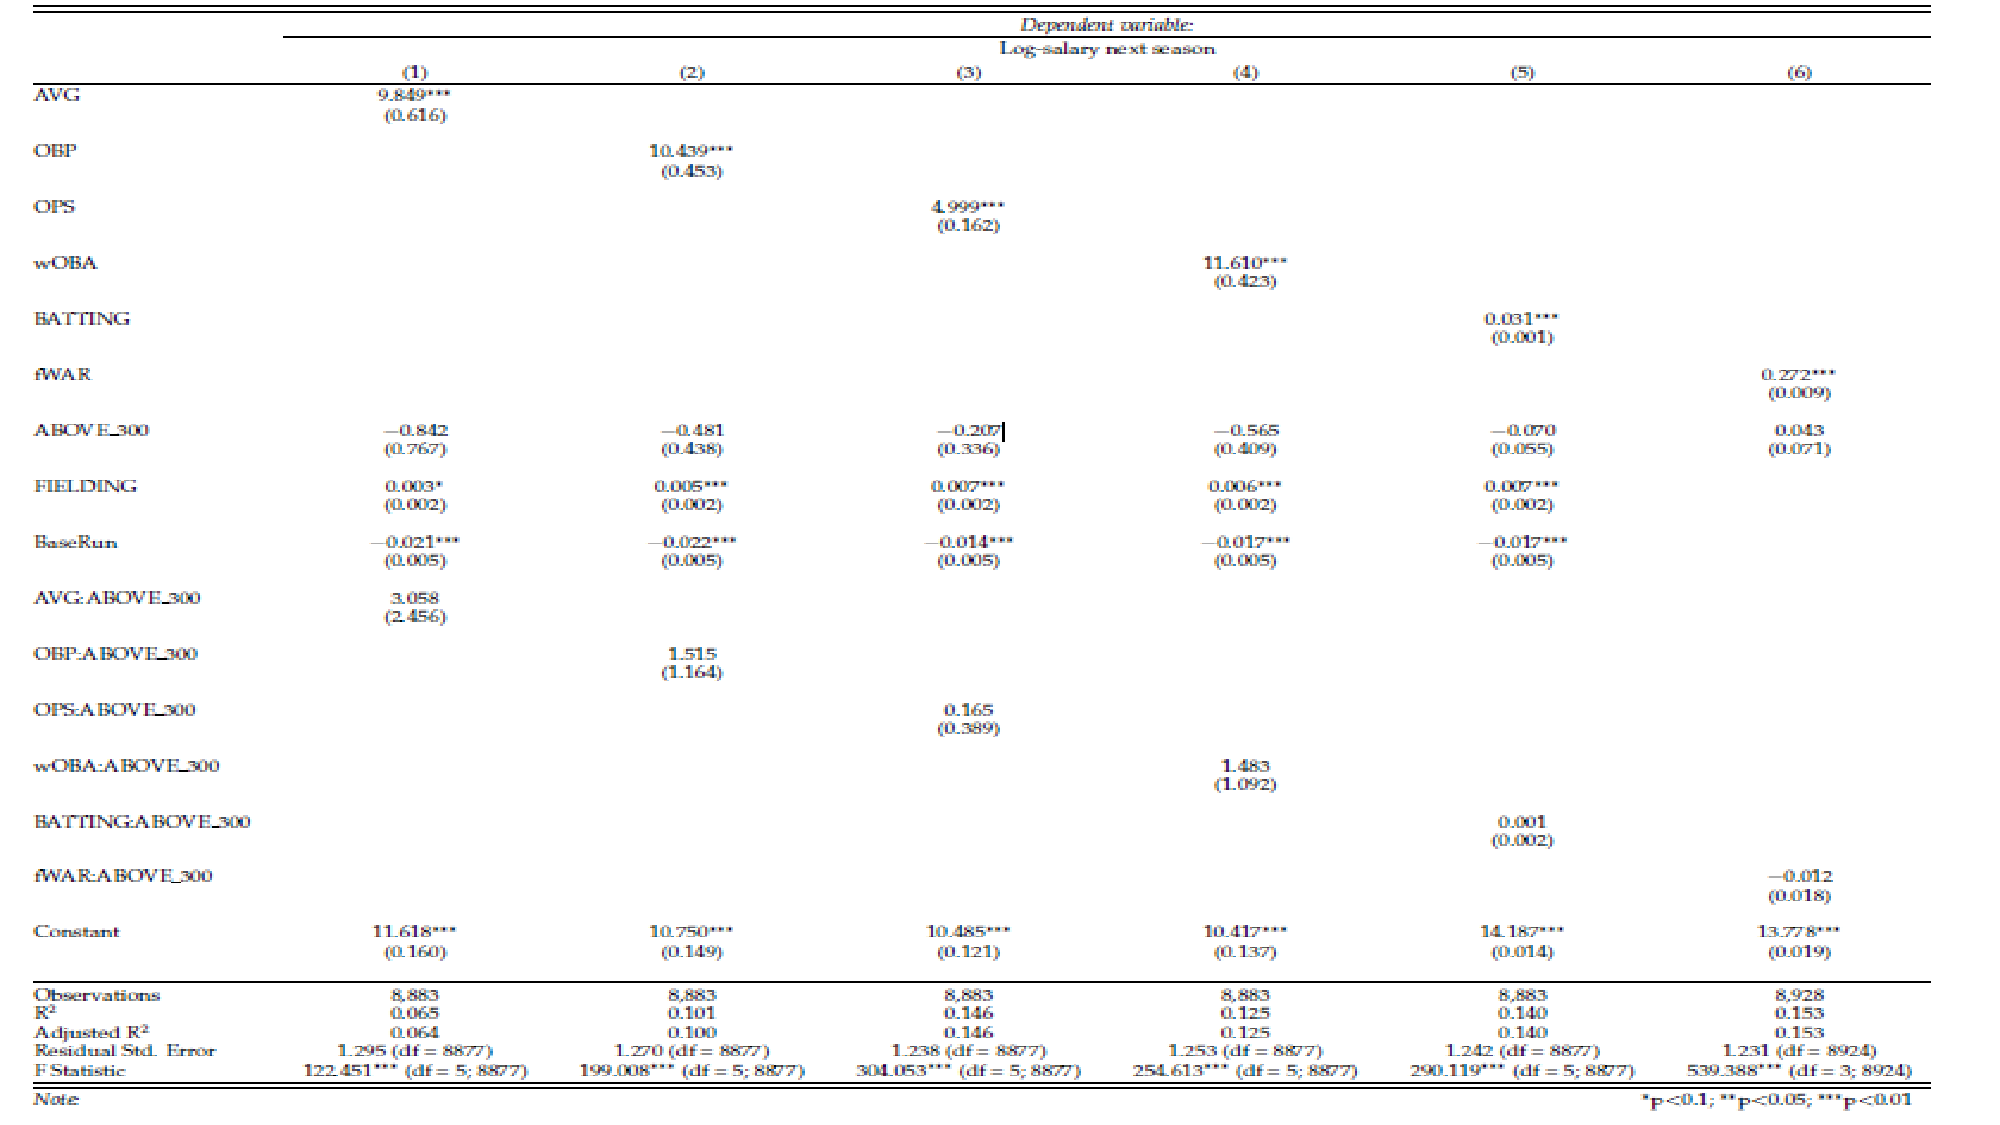
\includegraphics[width = 10cm, height = 8cm]{fig_tab/mt_tab1.pdf}
\label{}
 \end{figure}
\end{frame}

\begin{frame}
  \scriptsize
  performance = fWAR

  \begin{figure}
    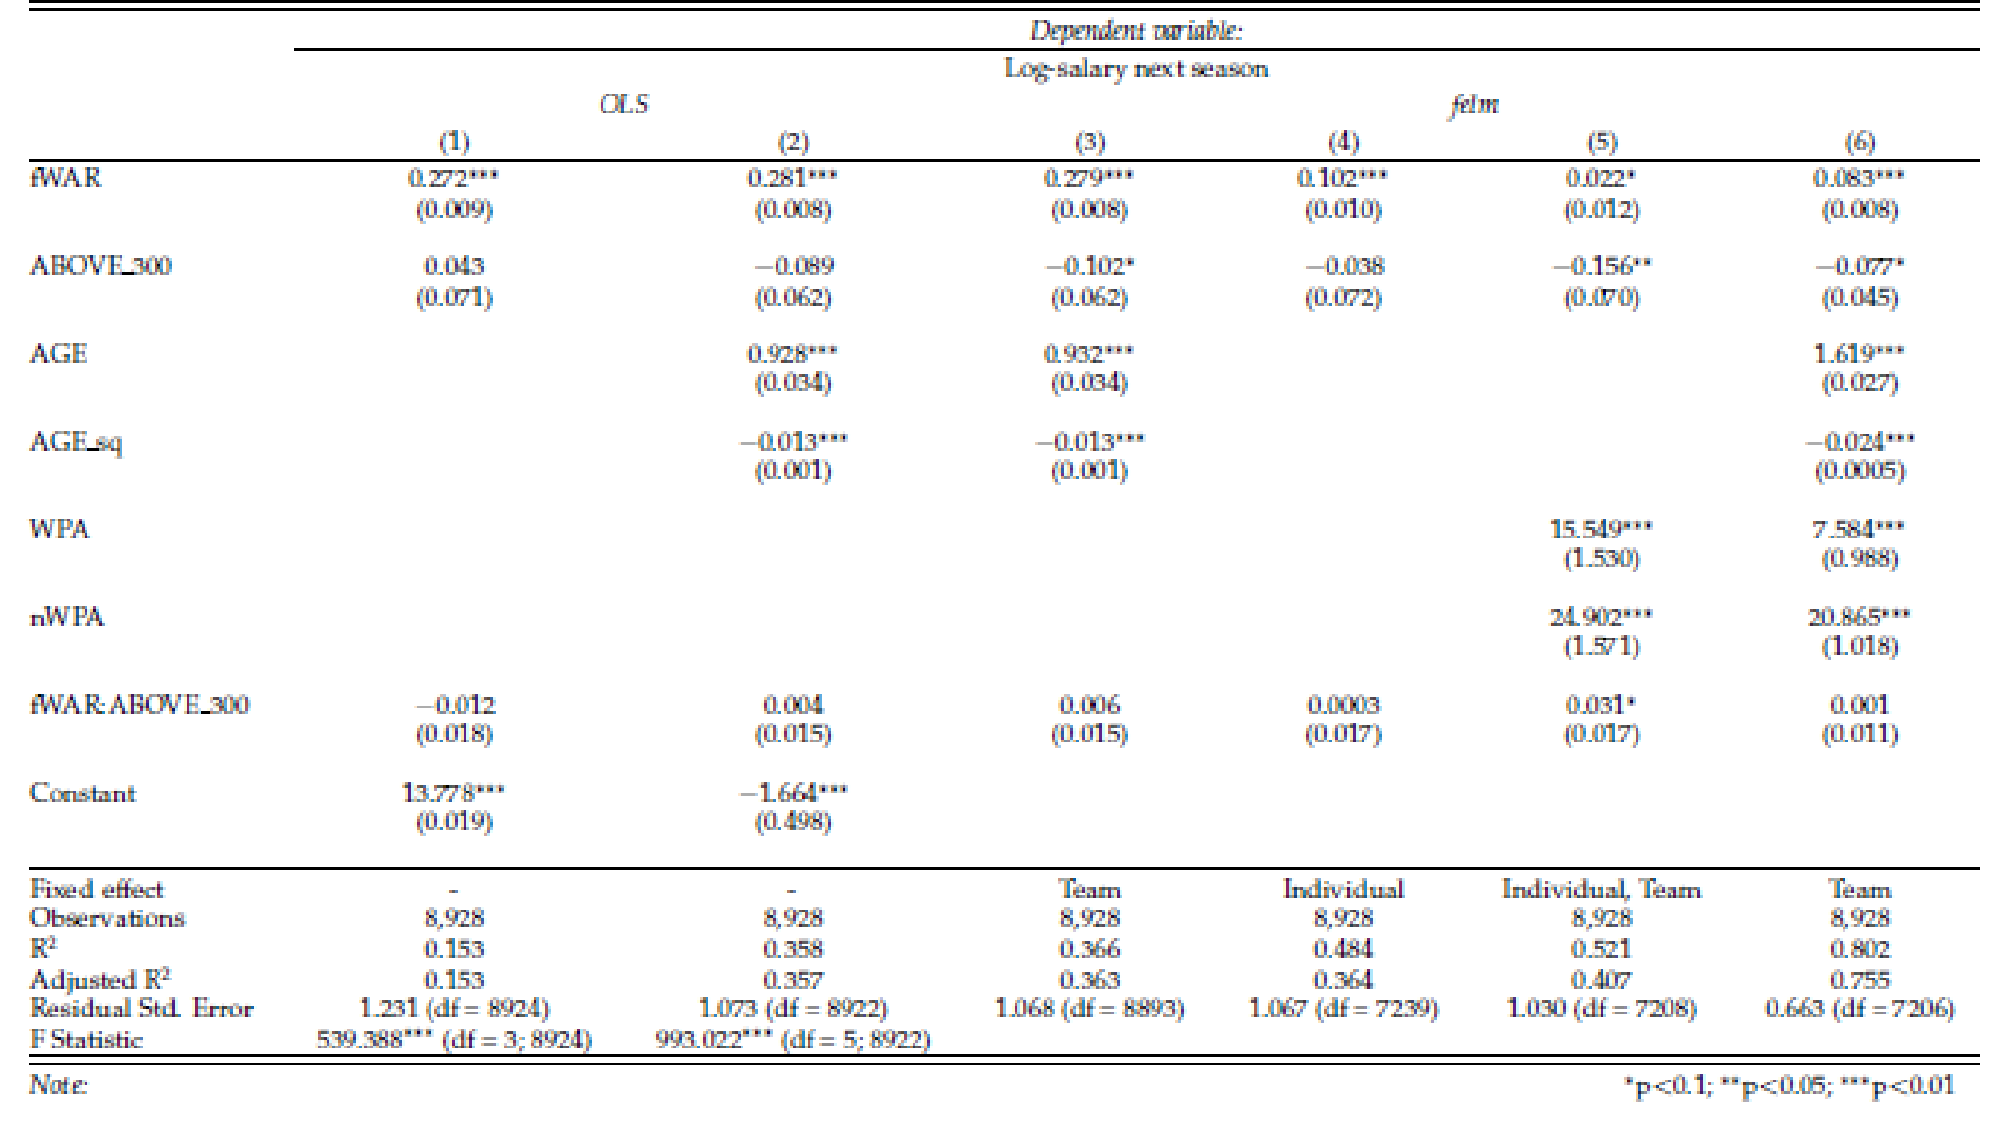
\includegraphics[width = 12cm, height = 8cm]{fig_tab/mt_tab2_0.pdf}
\label{}
  \end{figure}
\end{frame}

\begin{frame}
  \scriptsize
  performance = BATTING

  \begin{figure}
    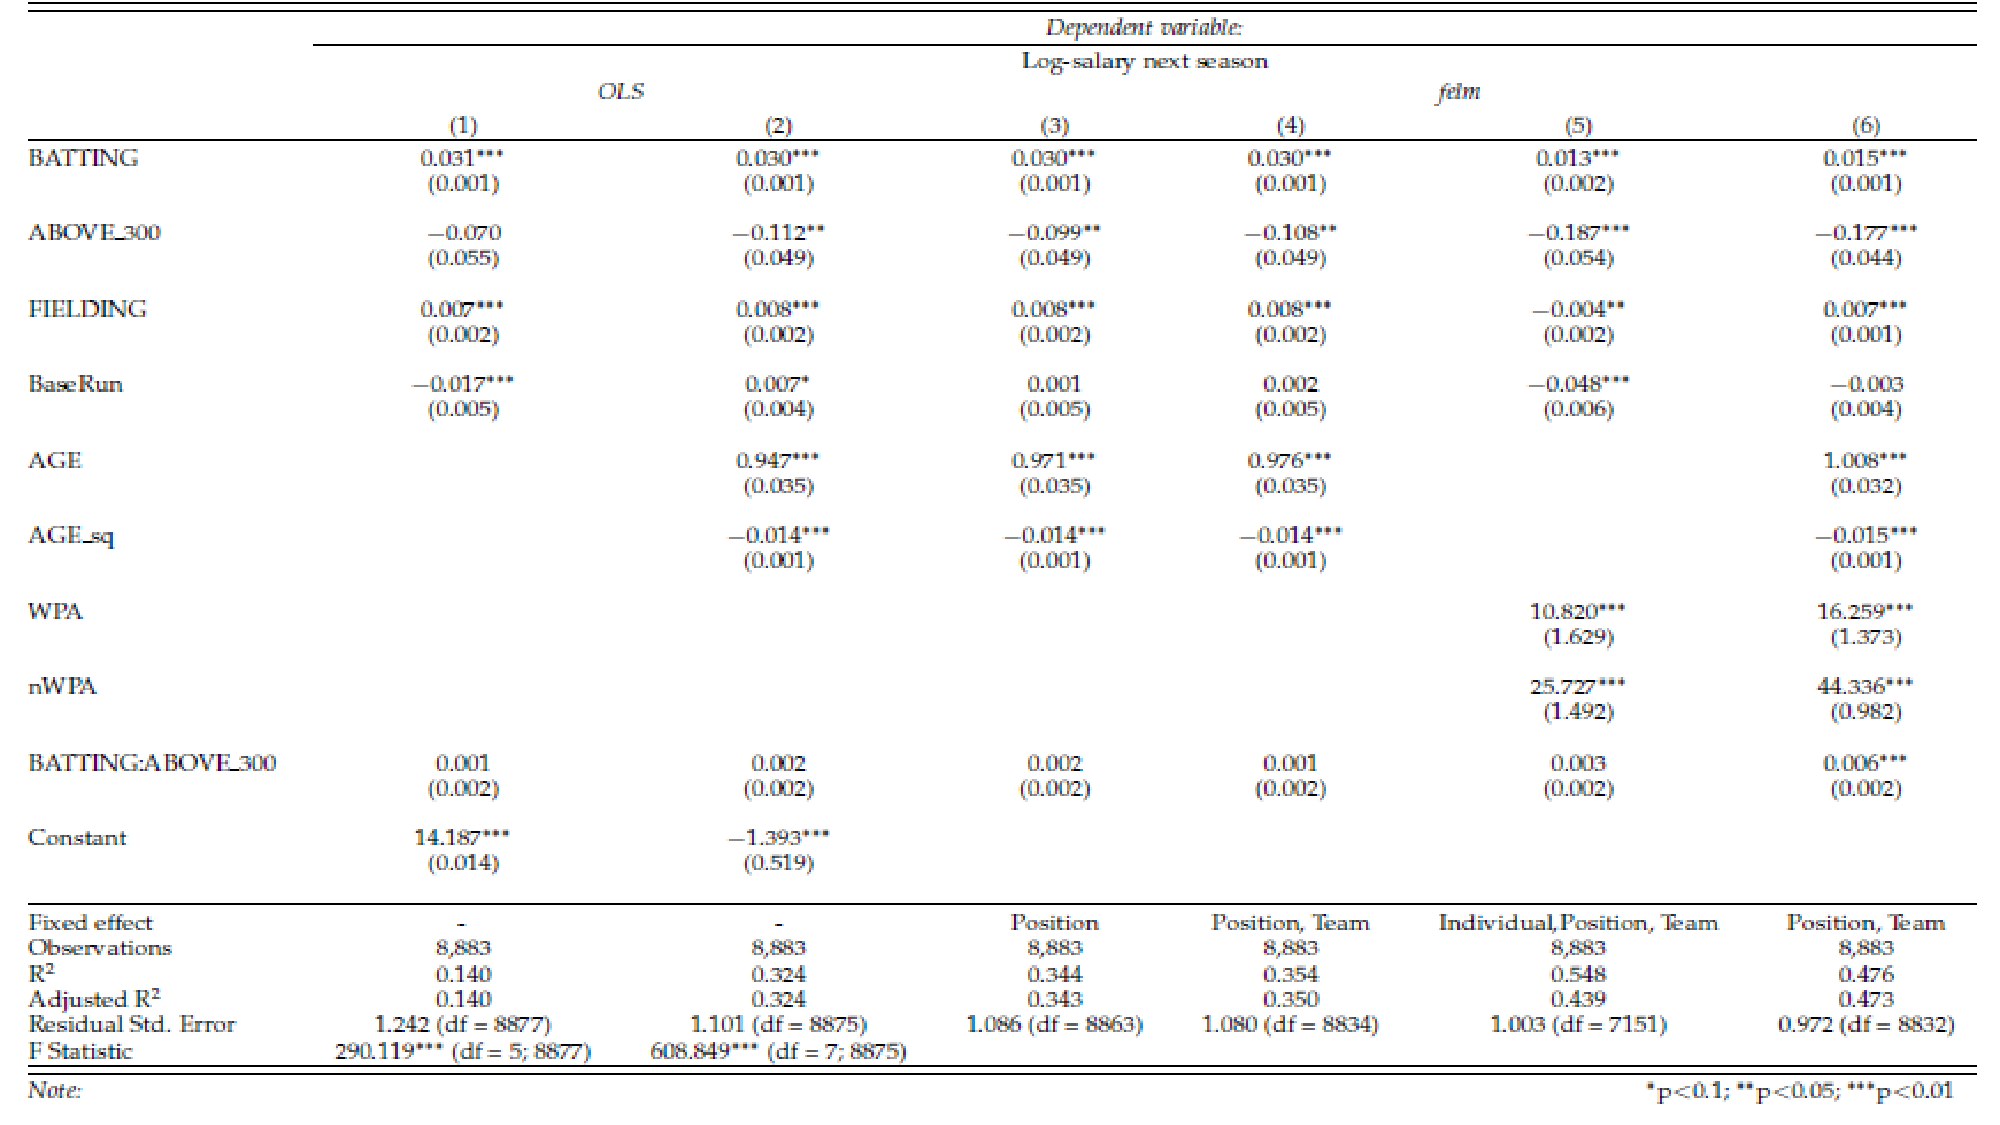
\includegraphics[width = 12cm, height = 8cm]{fig_tab/mt_tab2.pdf}
\label{}
  \end{figure}
\end{frame}

\begin{frame}\frametitle{\textit{`Moneyball'} Publication}
 \begin{itemize}
   \item `Moneyball' (Michael Lewis, 2003) claims that when it comes to
   measuring the performance from the viewpoint of how to score more runs and
   more wins, AVG is relatively less important statistics than On-base
   percentage or OPS (= OBP + SLG).

   \item Hakes \& Sauyer (2006) points out that MLB teams got to pay more to
   the players with high on-base percentage rather than batting average after
   the publication of \textit{Moneyball}.

   \item Reference dependence of the players may diminish after the model
   case of the \textit{Moneyball}, Oakland Athletics's World champion.

   \item Also, events that affects the procedure of the contraction may
   change the preference about the statistics.
 \end{itemize}
\end{frame}

\begin{frame}\frametitle{Classfying the Time series}
  I devide the sample into four eras:

  \begin{enumerate}
    \item Before ``Free Agent'' system was introduced: -1975
    ($n = 4292$)

    \item Before ``Strike'' of the players occurred: 1976-1994
    ($n = 5331$)

    \item Before `\textit{Moneyball}` was published: 1995-2001
    ($n = 2028$)

    \item After `\textit{Moneyball}`: 2002-
    ($n = 5555$)
  \end{enumerate}
\end{frame}

\begin{frame}
  \scriptsize


  \begin{figure}
    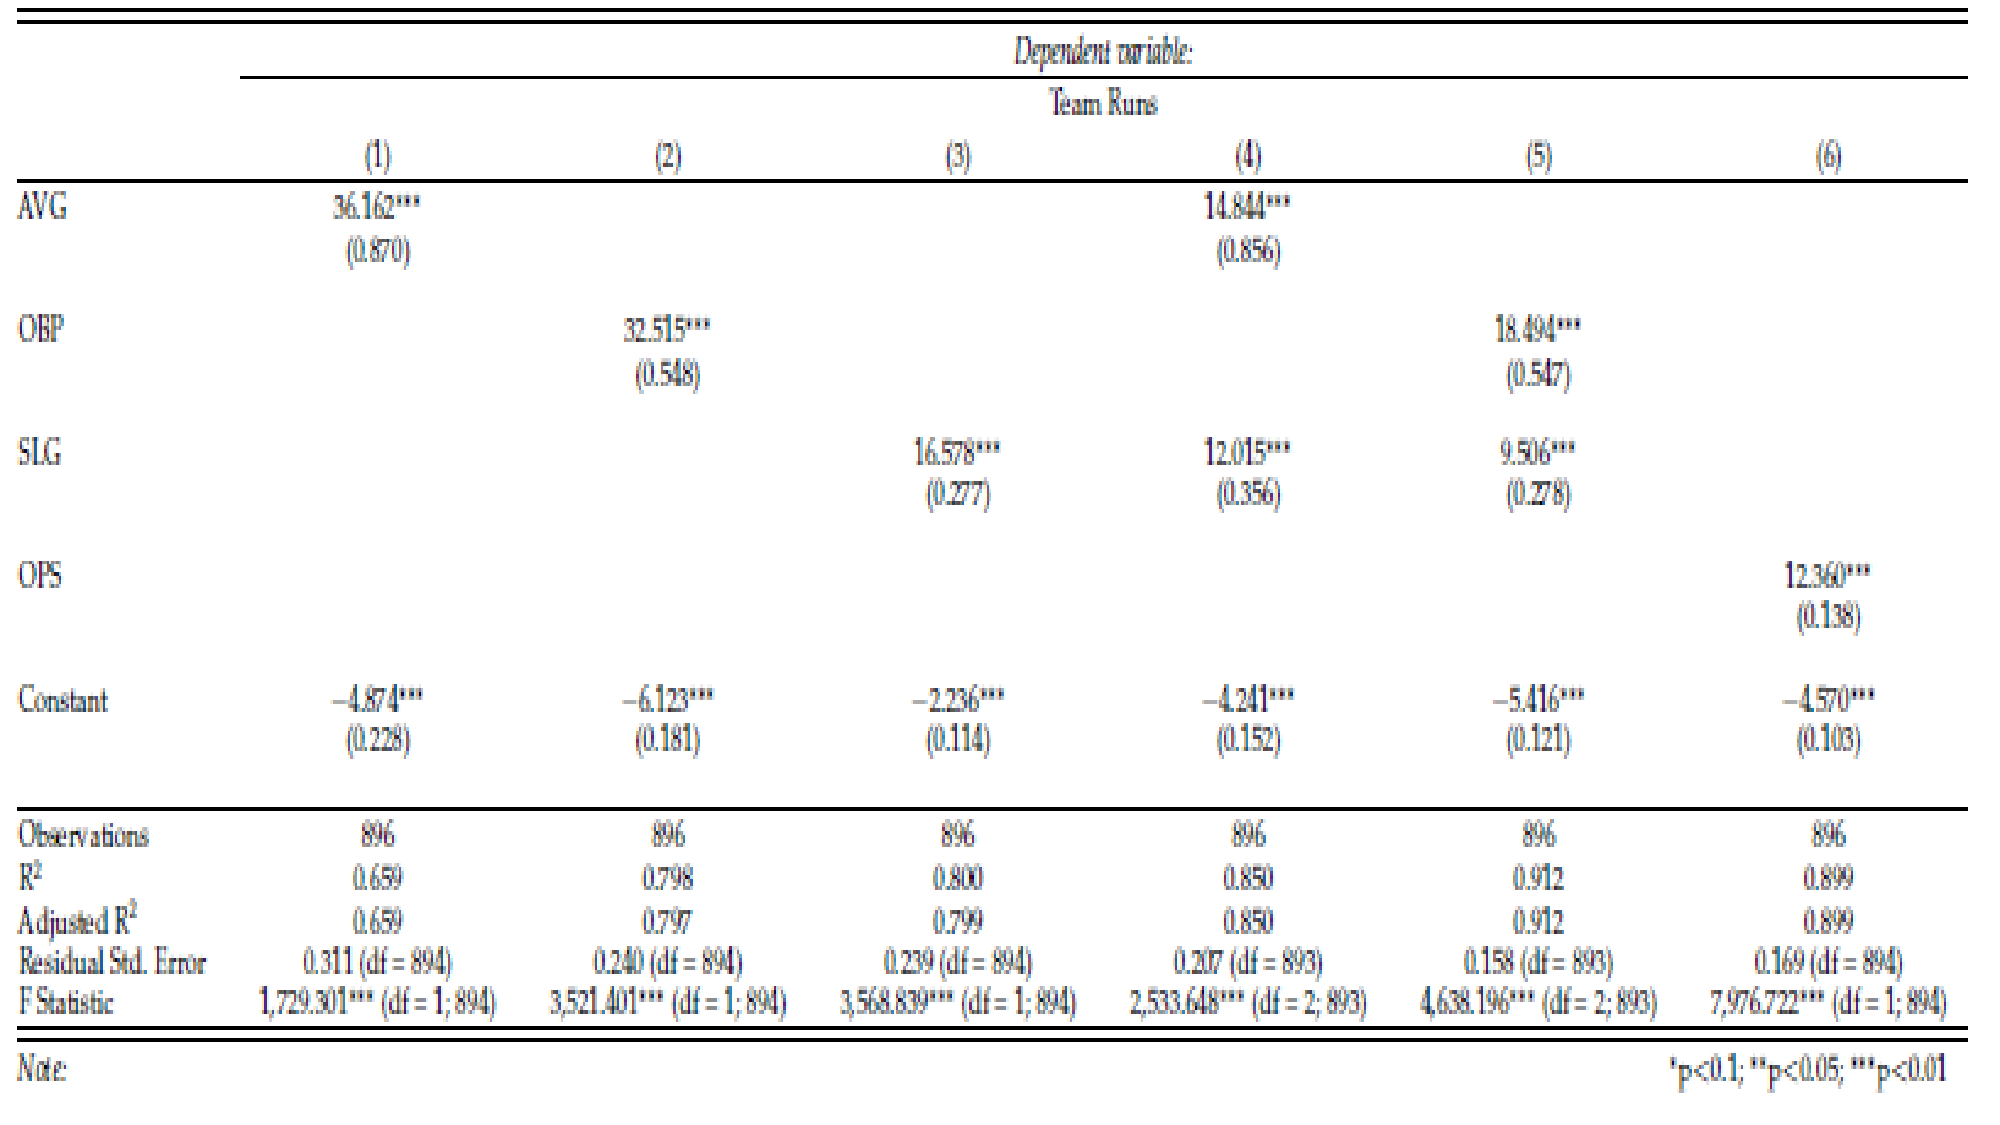
\includegraphics[width = 11cm, height = 5cm]{fig_tab/mt_tab7.pdf}
\label{}
  \end{figure}
\end{frame}

\begin{frame}

  \begin{figure}
    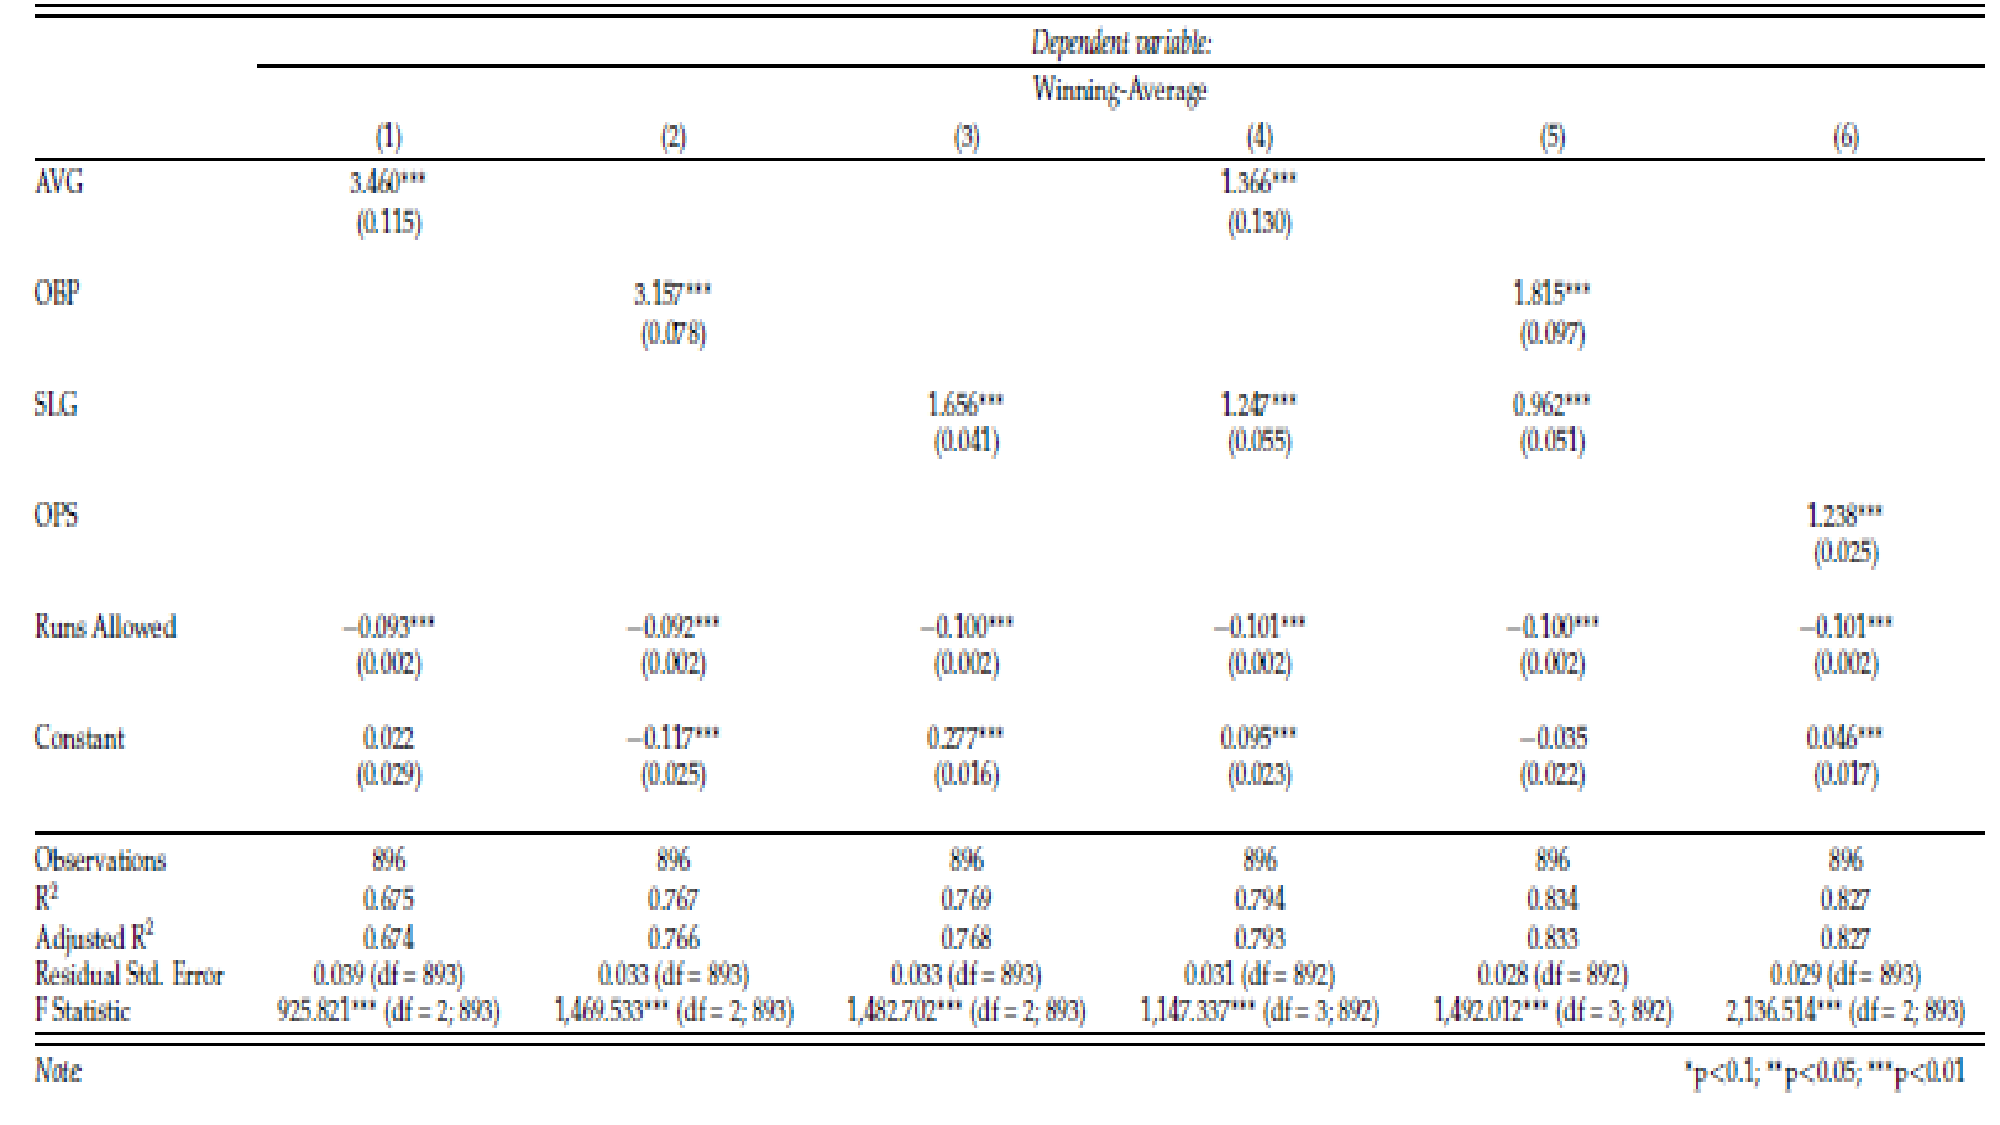
\includegraphics[width = 11cm, height = 5cm]{fig_tab/mt_tab8.pdf}
\label{}
  \end{figure}
\end{frame}

\begin{frame}
  \scriptsize
  Restricted sample for Before Strike

  \begin{figure}
    \includegraphics[width = 8.4cm, height = 6cm]
    {C:/Users/T-Reio/Master_thesis/master_thesis/graphs/AVG_bffa.png}
    \label{}
    \footnotesize

    .299 to .300: significant at 5\% ($\chi^2 = 3.04, p = 0.0406$)

   .298, .299 to .300, .301: significant at 1\% ($\chi^2 = 7.34, p = 0.0034$)
  \end{figure}
\end{frame}

\begin{frame}

  \begin{figure}
    \includegraphics[width = 8.4cm, height = 6cm]
    {C:/Users/T-Reio/Master_thesis/master_thesis/graphs/AVG_fast.png}
    \label{}
    \footnotesize

    .299 to .300: significant at 0.1\% ($\chi^2 = 31.88$)

   .298, .299 to .300, .301: significant at 0.1\% ($\chi^2 = 31.60$)
  \end{figure}
\end{frame}

\begin{frame}
  \begin{figure}
    \includegraphics[width = 8.4cm, height = 6cm]
    {C:/Users/T-Reio/Master_thesis/master_thesis/graphs/AVG_stmb.png}
    \label{}
    \footnotesize

    .299 to .300: significant at 0.1\% ($\chi^2 = 19.32$)

   .298, .299 to .300, .301: significant at 1\% ($\chi^2 = 7.28, p = 0.0034$)
  \end{figure}
\end{frame}

\begin{frame}
  \begin{figure}
    \includegraphics[width = 8.4cm, height = 6cm]
    {C:/Users/T-Reio/Master_thesis/master_thesis/graphs/AVG_afmb.png}
    \label{}
    \footnotesize

    .299 to .300: significant at 0.1\% ($\chi^2 = 16.67$)

   .298, .299 to .300, .301: significant at 0.1\% ($\chi^2 = 23.10$)
  \end{figure}
\end{frame}

\begin{frame}
  \begin{figure}
    \includegraphics[width = 8.4cm, height = 6cm]
    {C:/Users/T-Reio/Master_thesis/master_thesis/graphs/OBP_afmb.png}
    \label{}
  \end{figure}
\end{frame}

\begin{frame}
  \scriptsize
  Restricted sample for Before Strike

  performance = fWAR

  \begin{figure}
    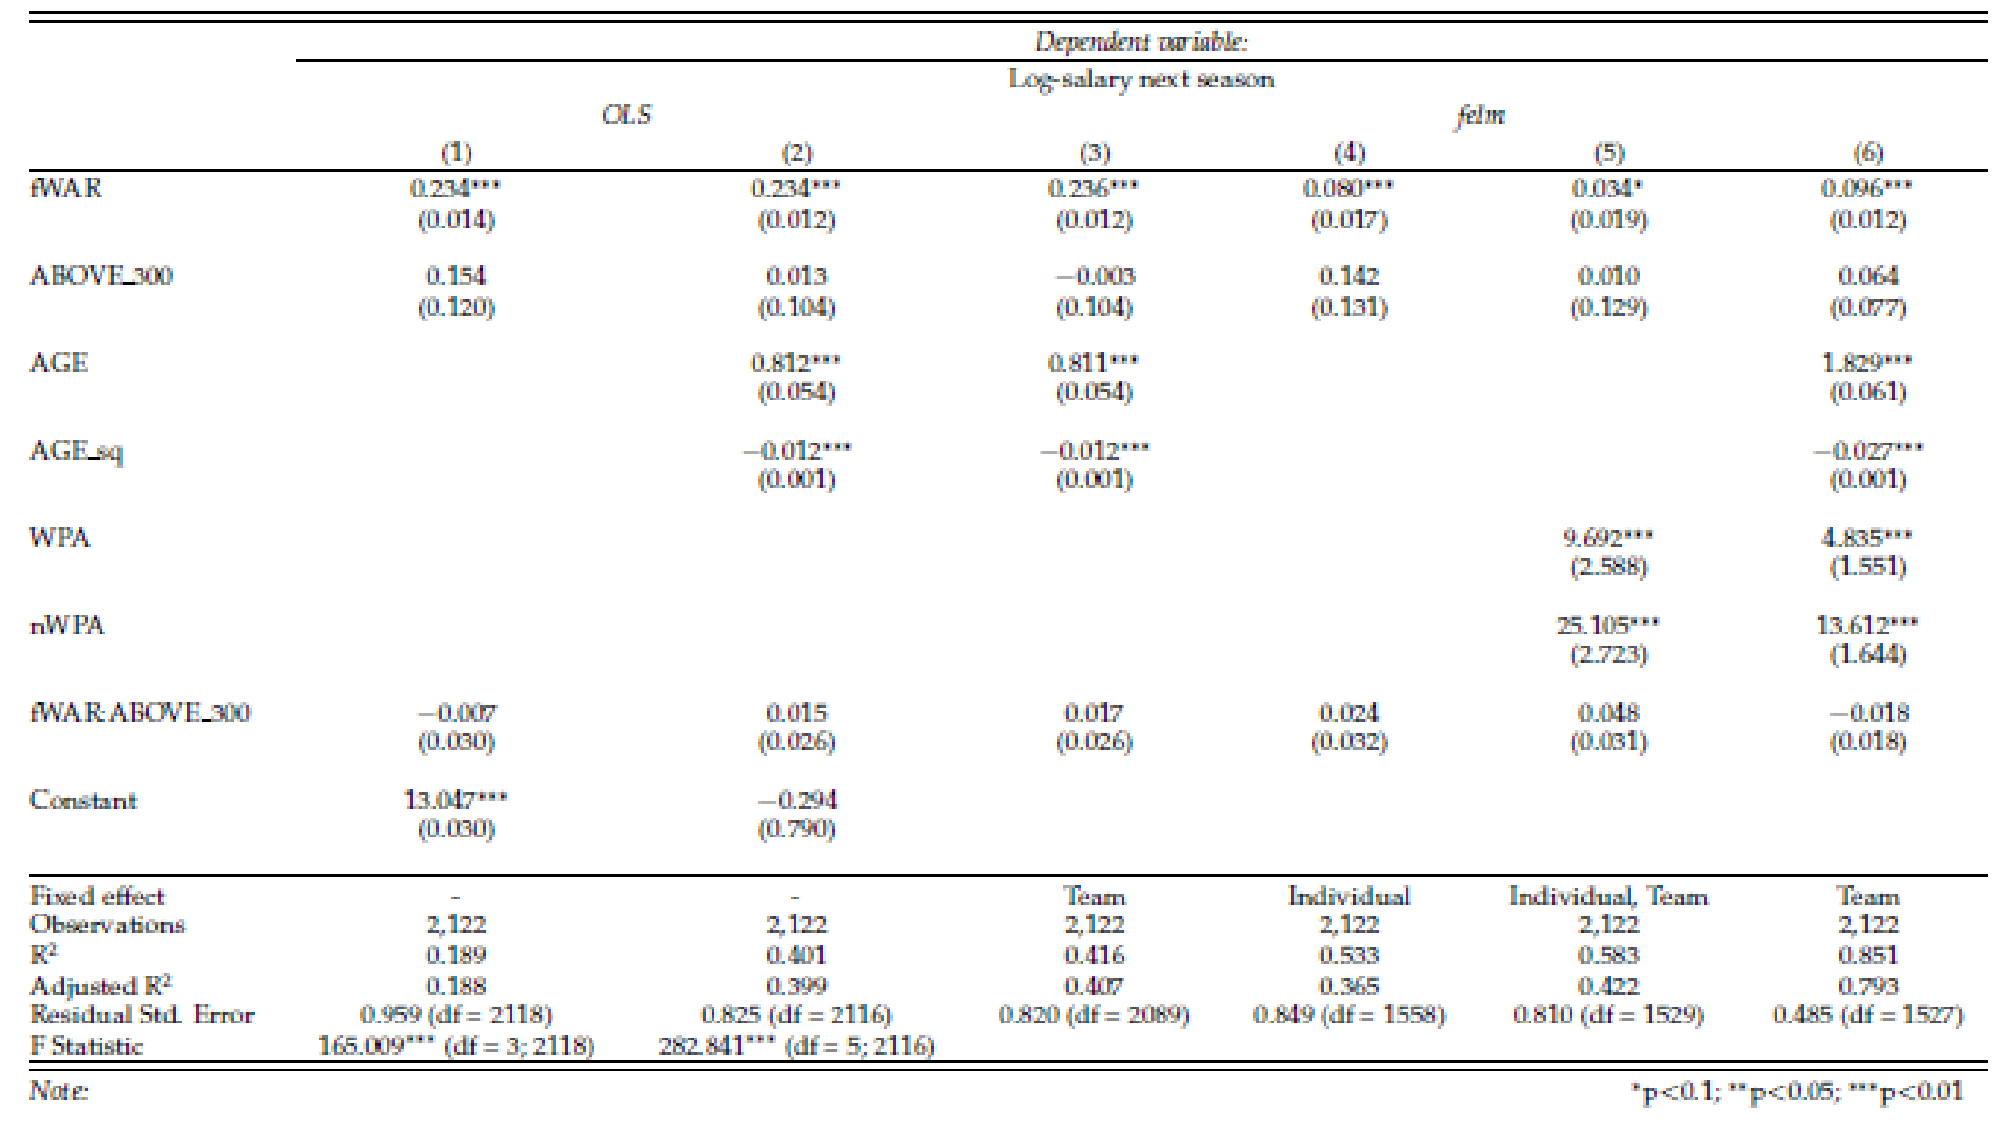
\includegraphics[width = 12cm, height = 8cm]{fig_tab/mt_tab3_0.pdf}
\label{}
  \end{figure}
\end{frame}

\begin{frame}
  \scriptsize
  Restricted sample for Before Strike

  performance = BATTING

  \begin{figure}
    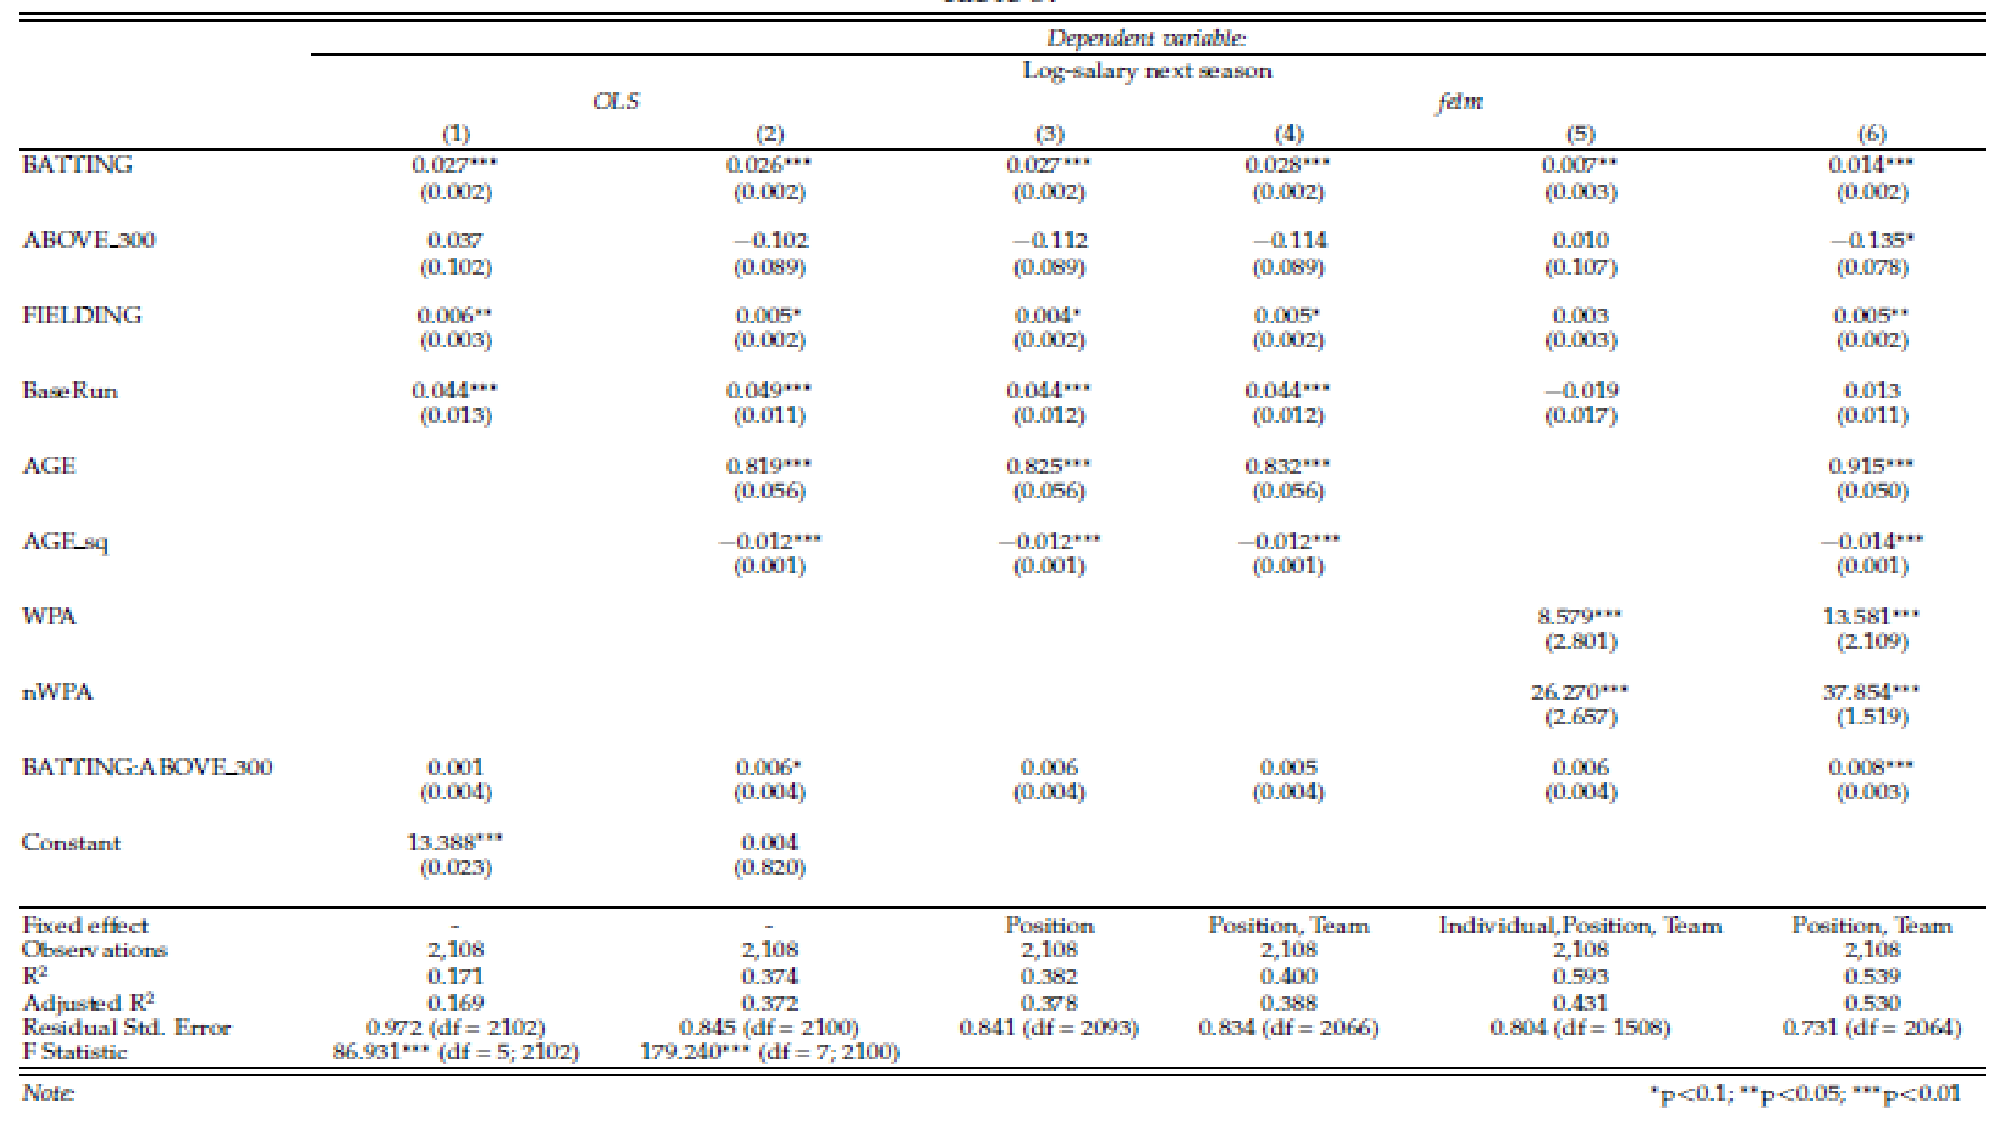
\includegraphics[width = 12cm, height = 8cm]{fig_tab/mt_tab3.pdf}
\label{}
  \end{figure}
\end{frame}

\begin{frame}
  \scriptsize
  Restricted sample for Before Moneyball

  performance = fWAR

  \begin{figure}
    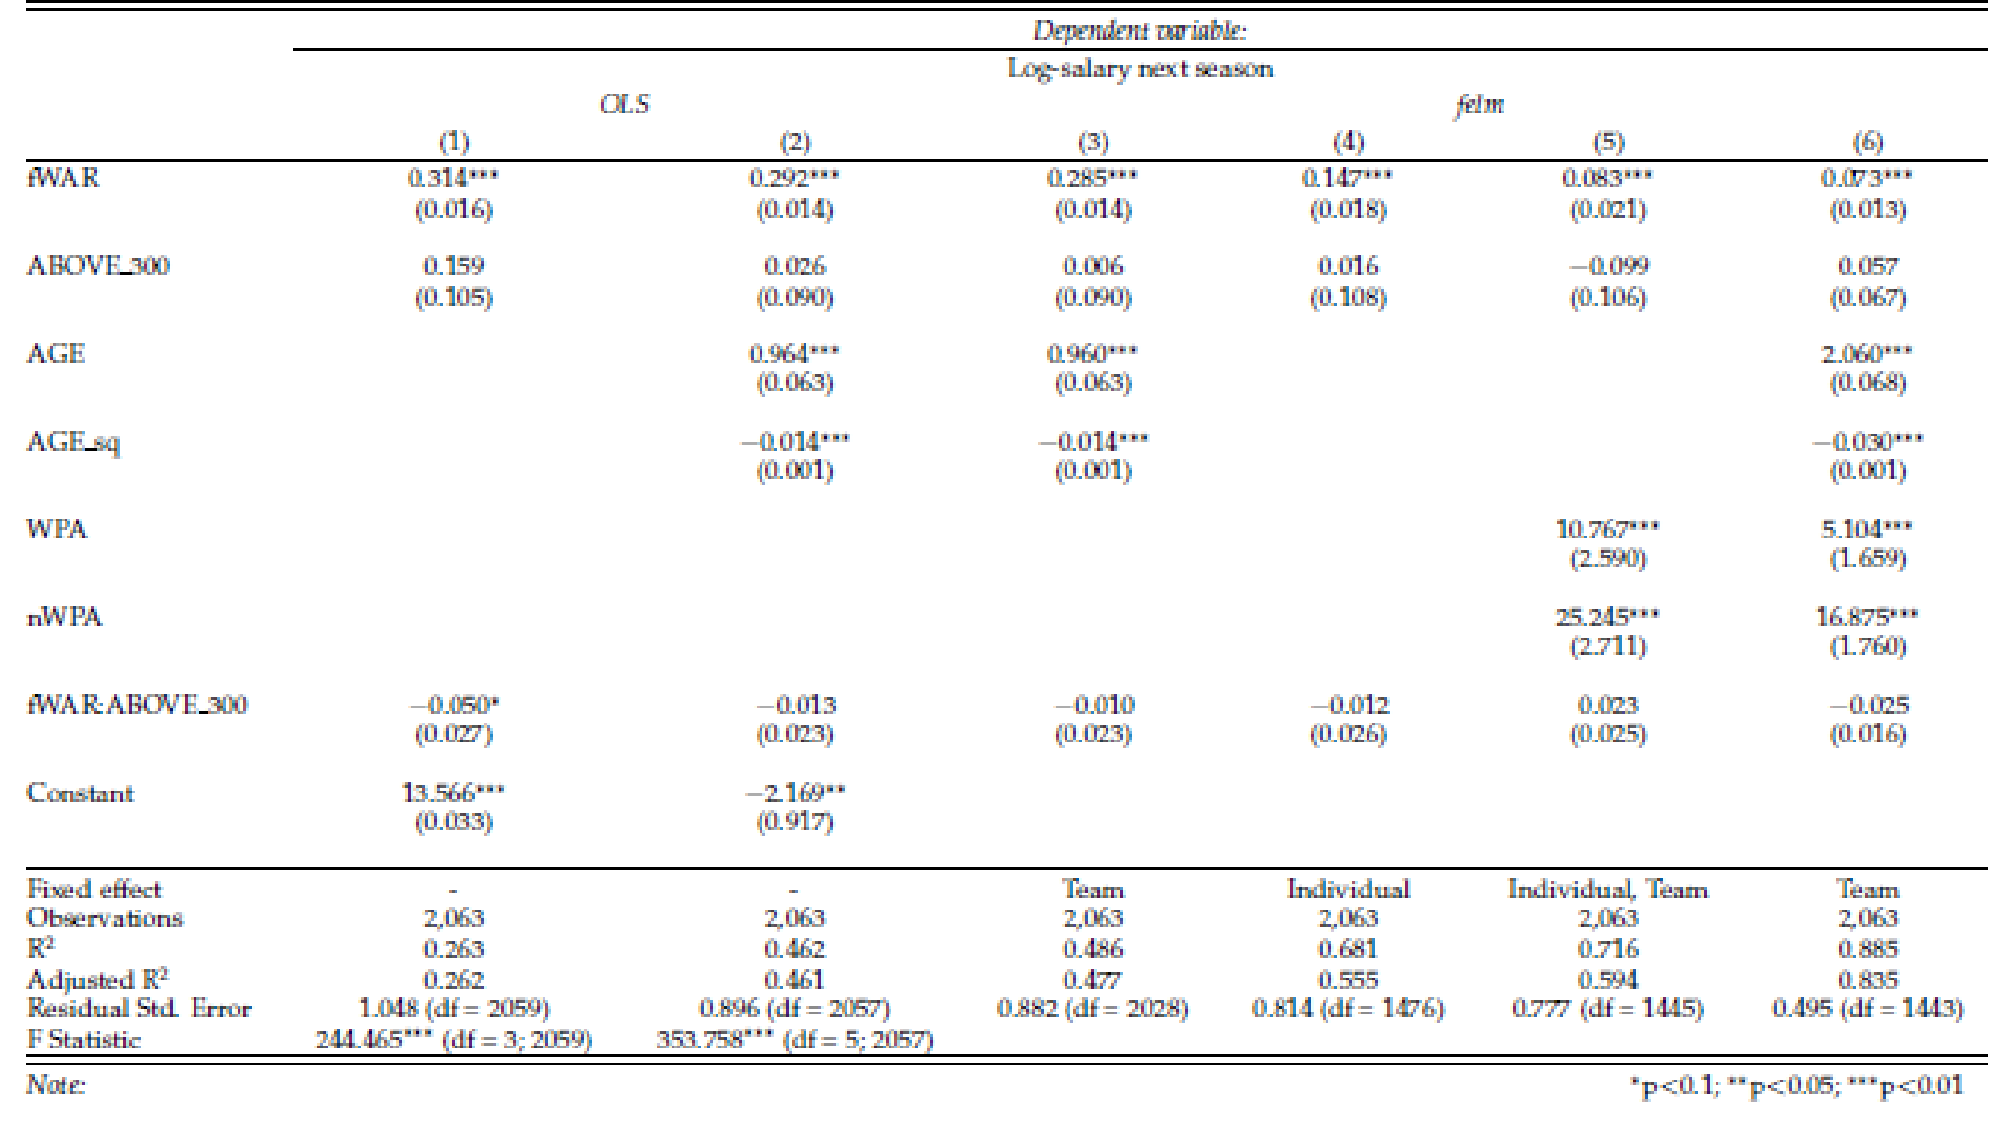
\includegraphics[width = 12cm, height = 8cm]{fig_tab/mt_tab4_0.pdf}
\label{}
  \end{figure}
\end{frame}

\begin{frame}
  \scriptsize
  Restricted sample for After Moneyball

  performance = BATTING

  \begin{figure}
    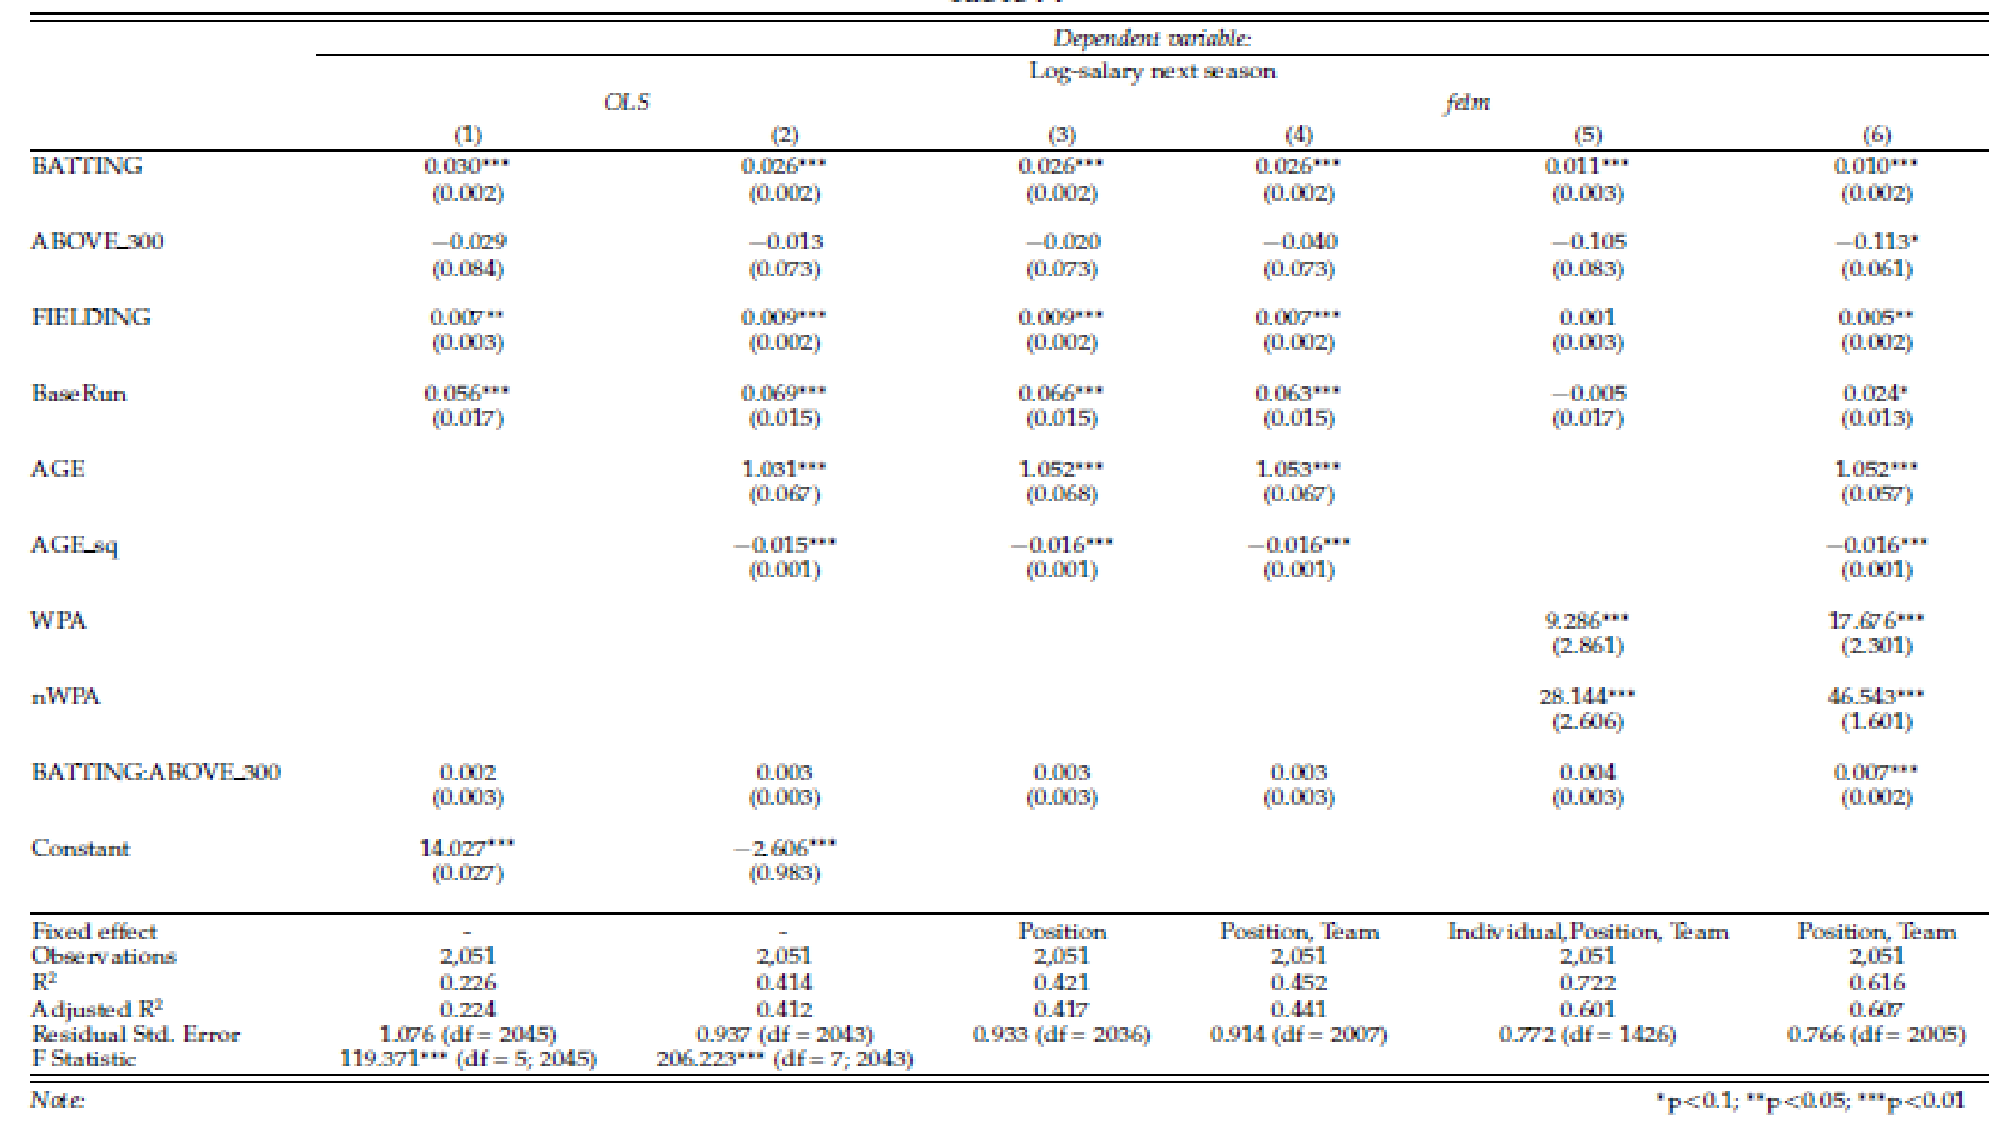
\includegraphics[width = 12cm, height = 8cm]{fig_tab/mt_tab4.pdf}
\label{}
  \end{figure}
\end{frame}

\begin{frame}
  \scriptsize
  Restricted sample for After Moneyball

  performance = fWAR

  \begin{figure}
    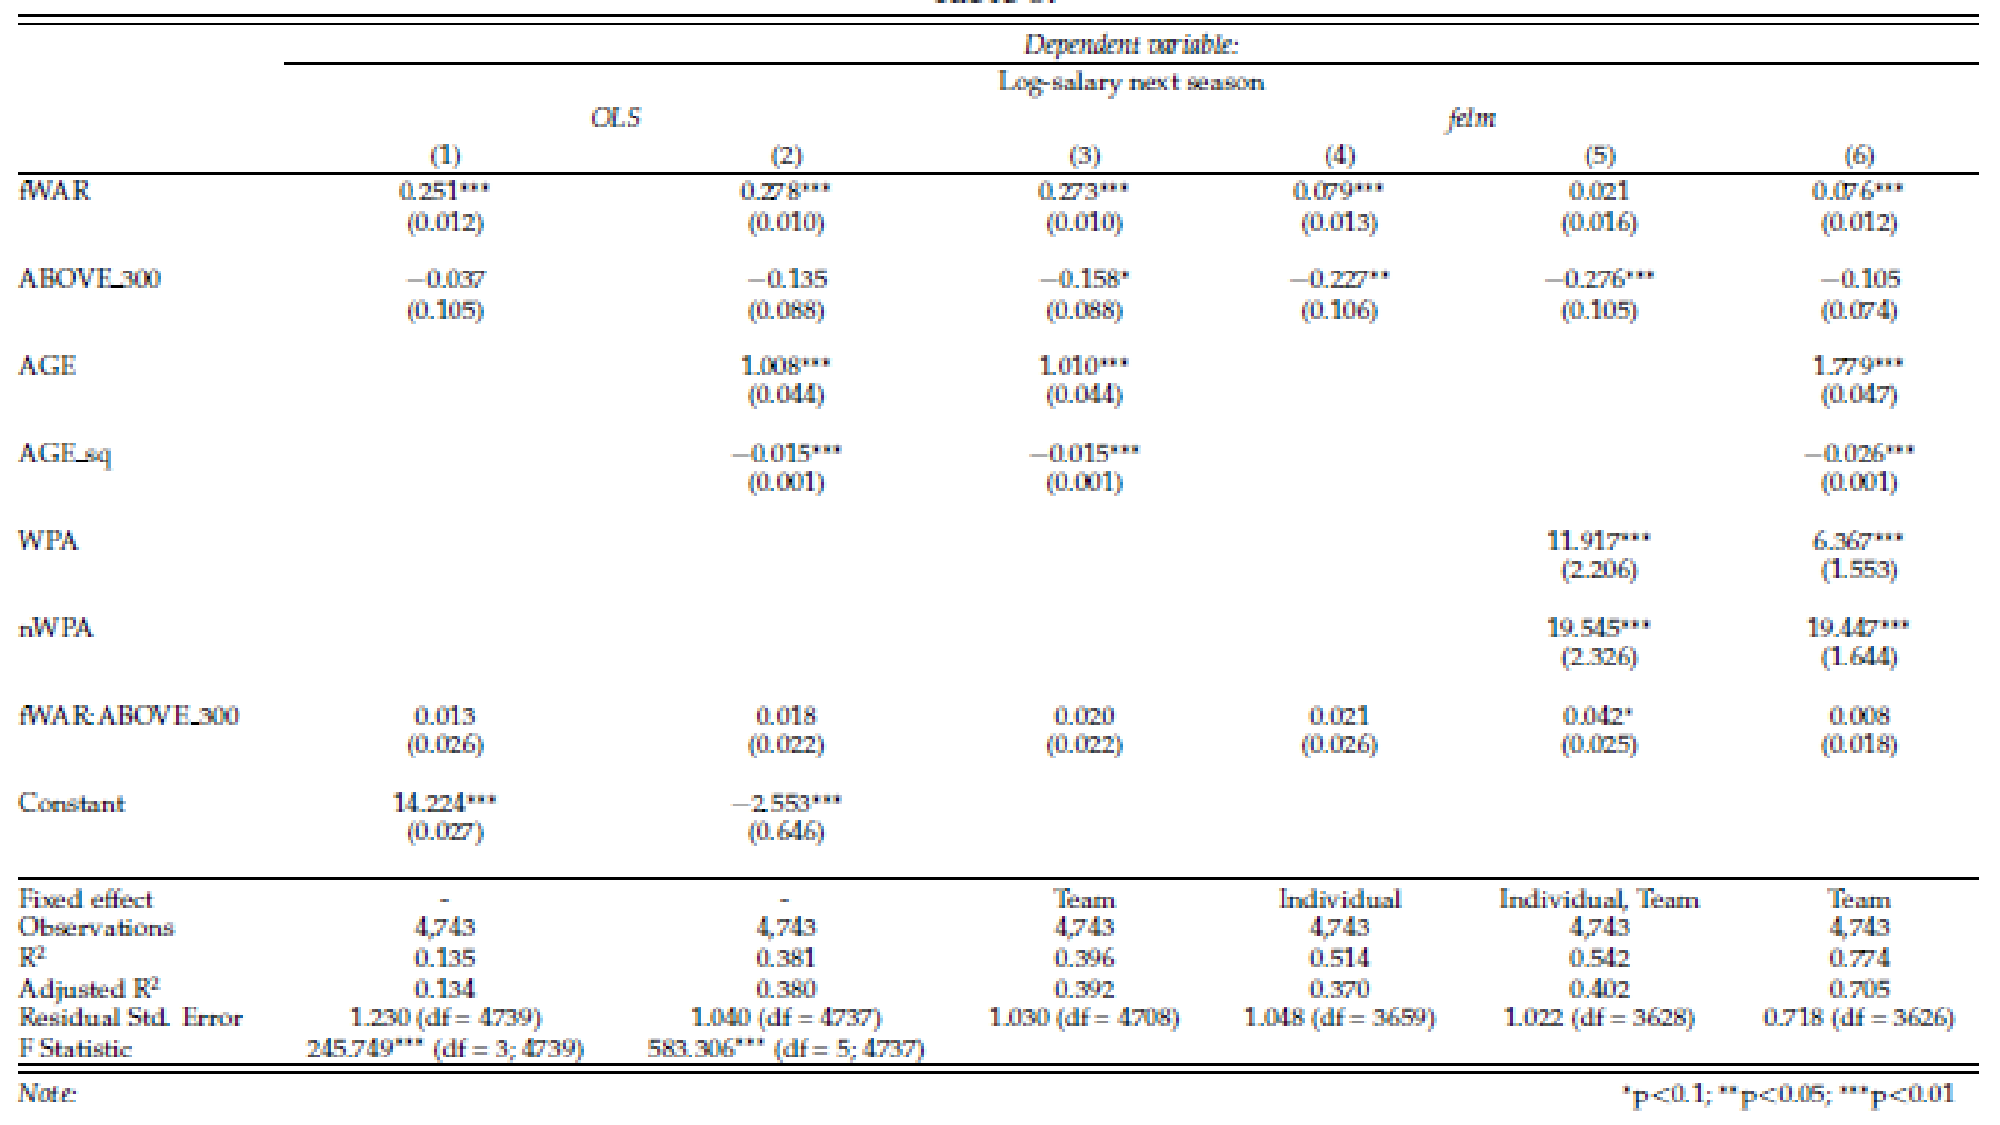
\includegraphics[width = 11cm, height = 8cm]{fig_tab/mt_tab5_0.pdf}
\label{}
  \end{figure}
\end{frame}

\begin{frame}
  \scriptsize
  Restricted sample for After Moneyball

  performance = BATTING

  \begin{figure}
    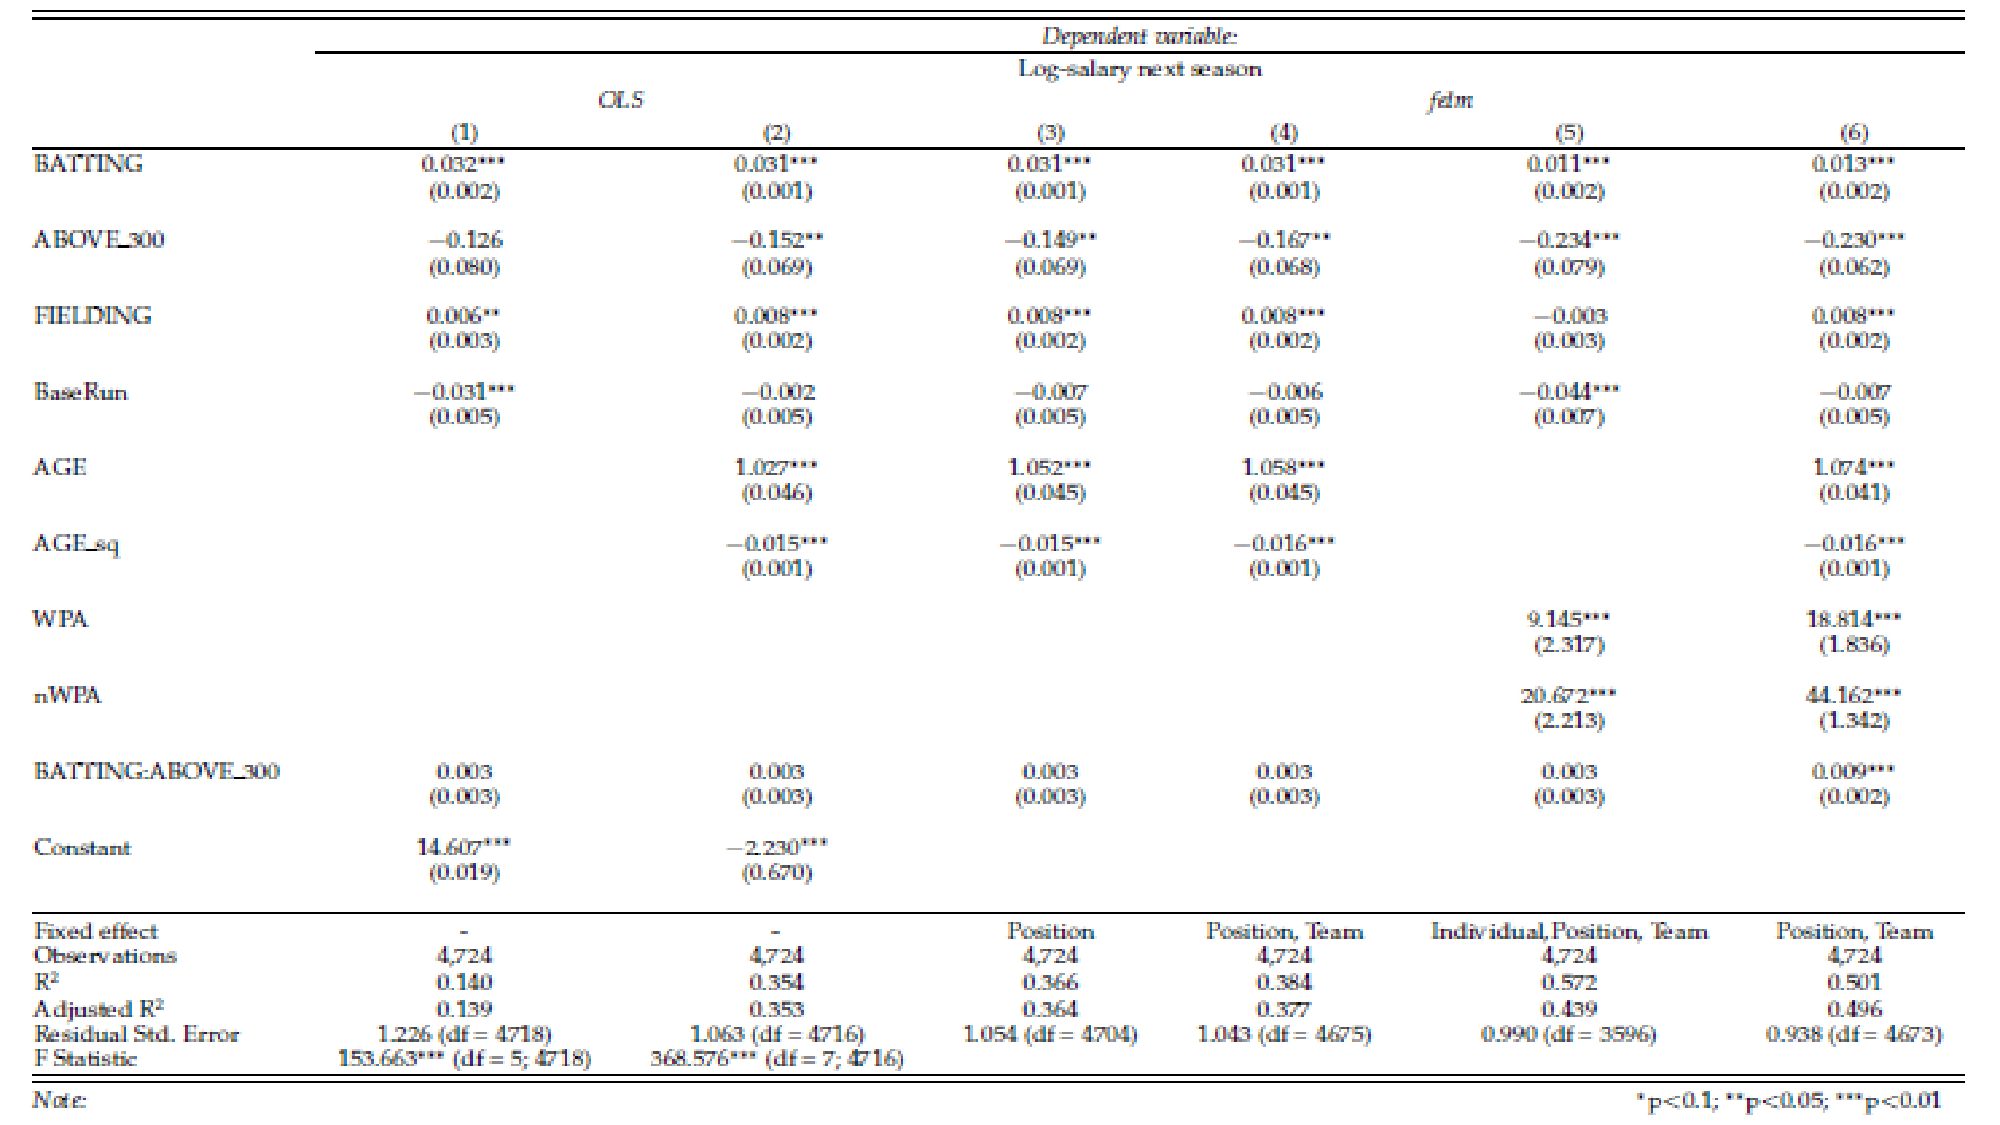
\includegraphics[width = 11cm, height = 8cm]{fig_tab/mt_tab5.pdf}
\label{}
  \end{figure}
\end{frame}

\begin{frame}
  \begin{figure}
    \scriptsize
    Full Sample:
    Including Era Dummies for Before Strike, Before Moneyball,
    and After Moneyball
    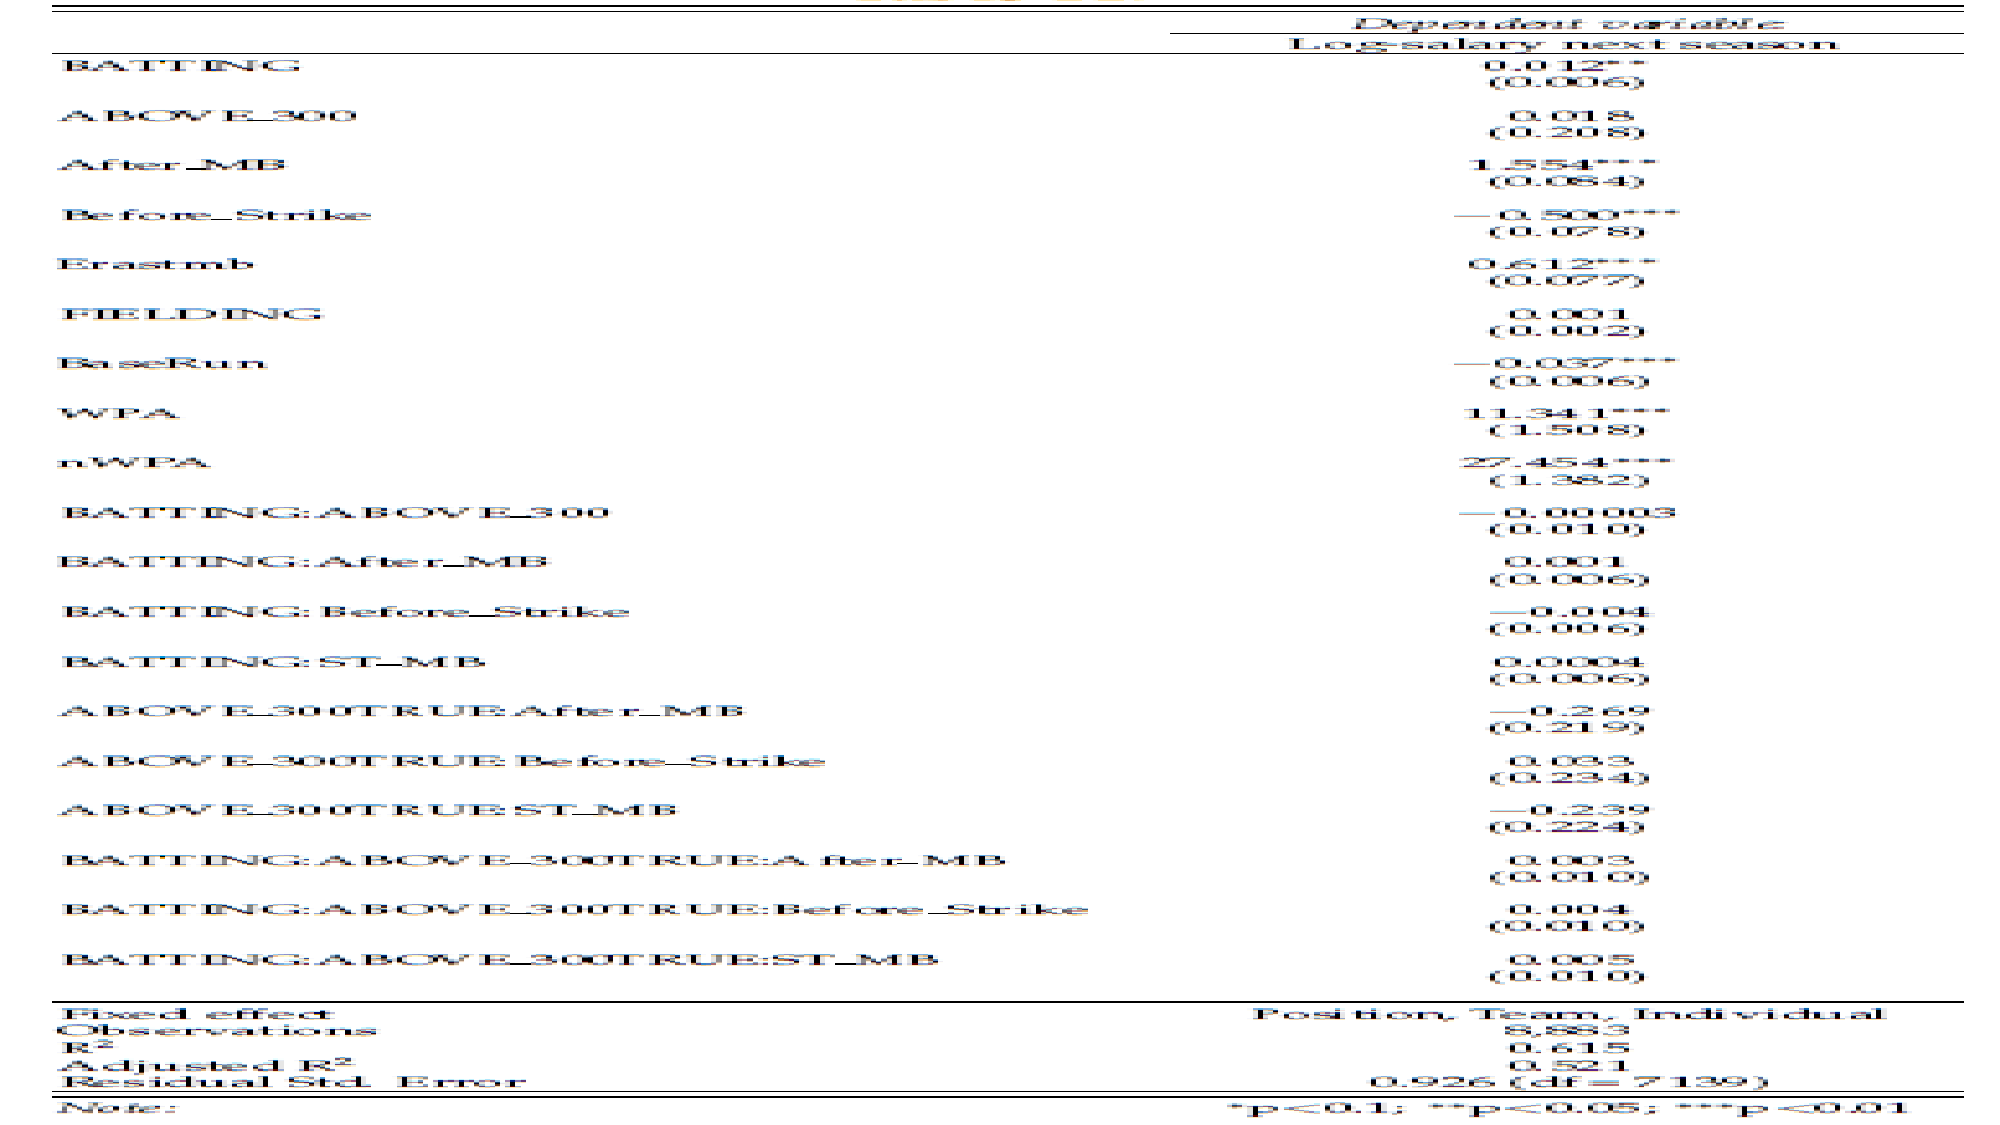
\includegraphics[width = 3cm, height = 8cm]{fig_tab/mt_tab6.pdf}

\label{}
  \end{figure}
\end{frame}

\section{Conclusion}
\begin{frame}\frametitle{Conclusion}
 \begin{itemize}
   \item Players regard .300 of batting-average as reference point:

   This preference is close to the evidence of Pope \& Schweizer (2011,AER),
   `` par " in the golf rather than ``round number."

   \item There are no monetary incentive that discontinuously raise their
   salary of them.

   \item Deipite of the evolution the technique of measuring the players'
   performance, they yet take batting-average important than other statistics
 \end{itemize}
\end{frame}

\begin{frame}\frametitle{Discussion}
  \begin{itemize}
    \item Round number reference dependence may diminish as the season
    get close to the end:

    See other knot of the season, such as at the All-Star game.

    \item How about career (= Not a single season) performance?

    \item Other elements of the contract can be monetary incentive:

    Additional bonus based on their performance contract length,
    possession of the right of free agent and arbitration


  \end{itemize}
\end{frame}

\section{Appendix}
\begin{frame}\frametitle{Specific Contents of the Contracts}
 from: \textit{Cot's Baseball Contracts}
  \begin{itemize}
    \item Adrian Beltre (Texas Rangers) 2011-2015, plus 2016
    \begin{itemize}
      \item voidable option

      \item Texas may void 2016 season if Beltre fails to
      reach 1,200 PAs in 2014-15 or 600 PAs 2015

      \item if option vests and Beltre is on Disabled List at end of
      2015 season and not healthy by spring 2016, club may defer
      \$12M of 2016 salary at 1\% interest

      \item award bonuses, including \$0.1M for each Gold Glove, All Star

      \item limited no-trade protection
    \end{itemize}
  \end{itemize}
\end{frame}

\begin{frame}\frametitle{Specific Contents of the Contracts}
\begin{itemize}
  \item Ichiro Suzuki (Seattle Mariners) 2001-2003
  \begin{itemize}
    \item \$5M signing bonus

    \item full no-trade clause

    \item performance bonuses:
     \begin{itemize}
       \item \$0.4M each for 200, 250, 300, 350, 450 PAs in 2001

       \item \$0.6M each for 200, 250, 300, 350, 450 PAs in 2003
     \end{itemize}

    \item award bonuses: \$0.15M for MVP
    (\$0.2M for 2nd award, \$0.25M for 3rd). \$0.1M for WS MVP.
     \$75,000 for Rookie of the Year. \$50,000 each for LCS MVP. Gold Glove,
      Silver Slugger. \$75,000 for most All-Star votes.
      \$50,000 for most All-Star votes in AL. \$50,000 for All-Star start.
       \$25,000 for All-Star reserve

    \item \$10,000 moving allowance, plus use of car, trainer, interpreter

    \item 2001-03 housing allowances: \$25,000, \$26,000, \$27,000

    \item four 1st-class air tickets between Japan & Seattle, twice a year
  \end{itemize}
\end{itemize}
\end{frame}

\begin{frame}\frametitle{References}
  \begin{itemize}
    \footnotesize
    \item Pope \& Simonsohn. 2011.
    Round Numbers as Goals: Evidence From Baseball, SAT Takers, and the Lab
    \textit{Psychological Science 22(1) 71–79}

    \item Hakes \& Sauer. 2006.
    An Economic Evaluation of the \textit{Moneyball} Hypothesis
    \textit{Journal of Economic Perspectives—Volume 20,
    Number 3—Summer 2006—Pages 173–185}

    \item Allen,Dechow, Pope \& Wu. 2016.
    Reference-Dependent Preferences: Evidence from
    Marathon Runners
    \textit{Management Science 63(6):1657-1672.}

    \item Pope \& Schweizer. 2011.
    Is Tiger Woods Loss Averse? Persistent Bias in the
    Face of Experience, Competition, and High Stakes
    \textit{American Economic Review 101 (February 2011): 129–157}

    \item Kahneman \& Tversky.1979.
    Prospect Theory: An Analysis of Decision under Risk.
    \textit{Econometrica:  Journal of the Econometric Society47 (2): 263–291.}

  \end{itemize}
\end{frame}

\begin{frame}\frametitle{Data References}
  \begin{itemize}
    \item fangraphs Baseball

    https://www.fangraphs.com/

    \item Baseball Reference

    https://www.baseball-reference.com

    \item USA TODAY

    https://www.usatoday.com/sports/mlb/

    \item Baseball Prospectus

    https://www.baseballprospectus.com/
  \end{itemize}
\end{frame}
\end{document}
